\chapter{Results and Discussion}

\section{SCAN vs.\ r$^2$SCAN functional}
In order to perform deep neural network training, one must first label the dataset using DFT. Implementing DFT calculations requires selecting appropriate parameters, such as the exchange-correlation functional. Water is a delicate molecule, sensitive to the complex competition between attractive interactions (e.g., hydrogen bonds, covalent bonds, and van der Waals forces), which bring order, and thermal fluctuations, which introduce disorder into the system. Numerous studies have attempted to describe this delicate nature of water. One promising functional is the Strongly Constrained and Appropriately Normed (SCAN) density functional, which is a non-empirical semilocal meta-GGA functional that satisfies all 17 known exact constraints and is appropriately normed on systems for which a semilocal functional can be exact or extremely accurate~\cite{sun2015strongly}. SCAN is not fitted to any bonded system, yet it predicts certain bonding properties very well, such as atomization energies, weak-interaction binding energies, and lattice constants of solids, although it does not predict energy barriers to chemical reactions. It has been shown that SCAN accurately describes covalent bonds, hydrogen bonds, and van der Waals interactions, which play important roles in the structure and dynamics of liquid water~\cite{chen2017ab}. It is also one of the functionals that predict ice as less dense than liquid water under standard conditions. Unfortunately, imposing rigid constraints can cause numerical instabilities, as we observed when applying SCAN to systems with interfaces. Instead, this study used a similar but more accurate and numerically efficient regularized-restored r$^2$SCAN meta-generalized gradient approximation~\cite{Furness2020}. The r$^2$SCAN functional is based on the previously proposed rSCAN functional, which regularizes or relaxes some of the constraints of SCAN to improve numerical performance~\cite{bartok2019}. The r$^2$SCAN functional restores these constraints but with a more consistent error in grid density, requiring smaller grids to achieve good accuracy.

We conducted a comparison between the SCAN and r$^2$SCAN exchange-correlation functionals to determine the extent of the discrepancy between the two. Figures~\ref{fig:scan_r2scan_E} and~\ref{fig:scan_r2scan_F} show that the total relative energy and atomic forces are in good agreement between the two functionals. The computed root mean square error of the forces was 0.048 \unit{eV/\angstrom}, which is of the same magnitude as typical validation errors in ML models. See Figure~\ref{fig:scan_r2scan_F_dist} for the distribution plot of the error in forces. Convergence tests were conducted to determine the appropriate energy cut-offs for the DFT calculations. As shown in Figures~\ref{fig:conv_scan} and~\ref{fig:conv_r2scan}, a cutoff of 130 Ry is adequate for convergence on energy, force, and pressure for both the SCAN and r$^2$SCAN functionals. This is also consistent with what Chen et al.~\cite{chen2017ab} used in their modeling of water.

\begin{figure}[tbhp]
	\centering
	\begin{subfigure}{0.48\textwidth}
		\centering

		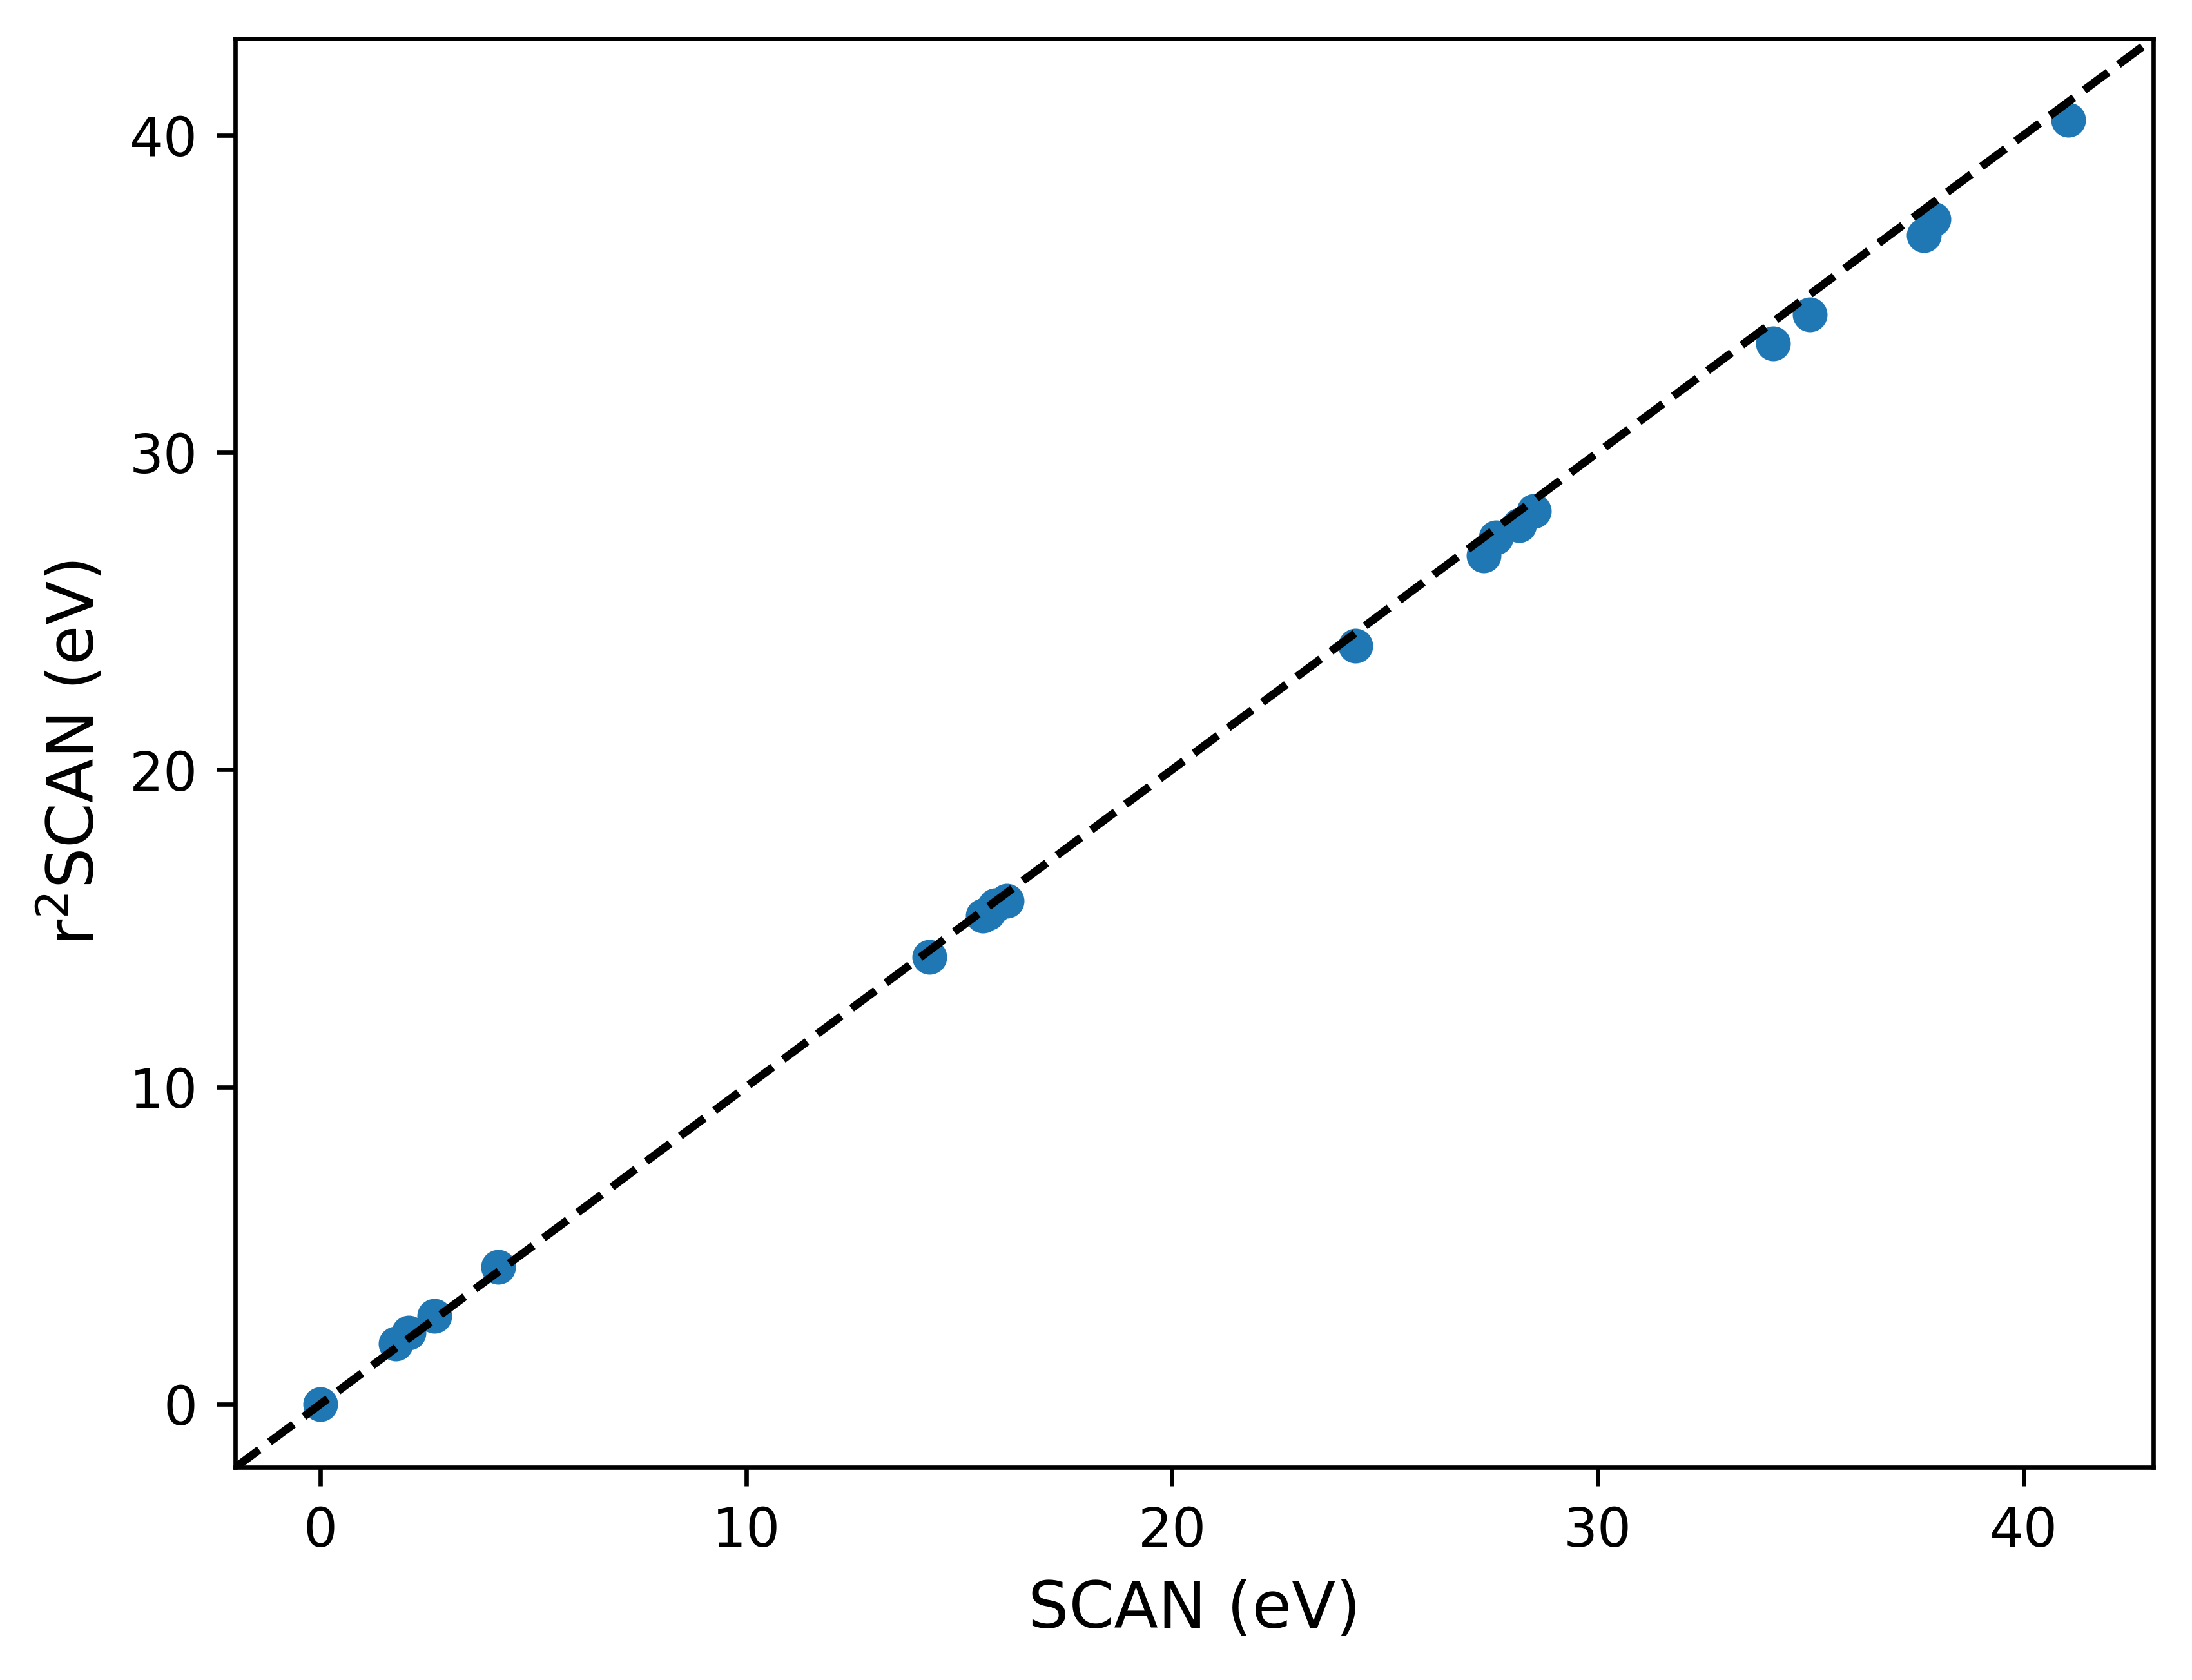
\includegraphics[width=0.9\textwidth]{images/scan_vs_r2scan/energy_compare.png}
		\caption{Relative Total Energy Comparison}\label{fig:scan_r2scan_E}
	\end{subfigure}
	\hfill
	\begin{subfigure}{0.48\textwidth}
		\centering

		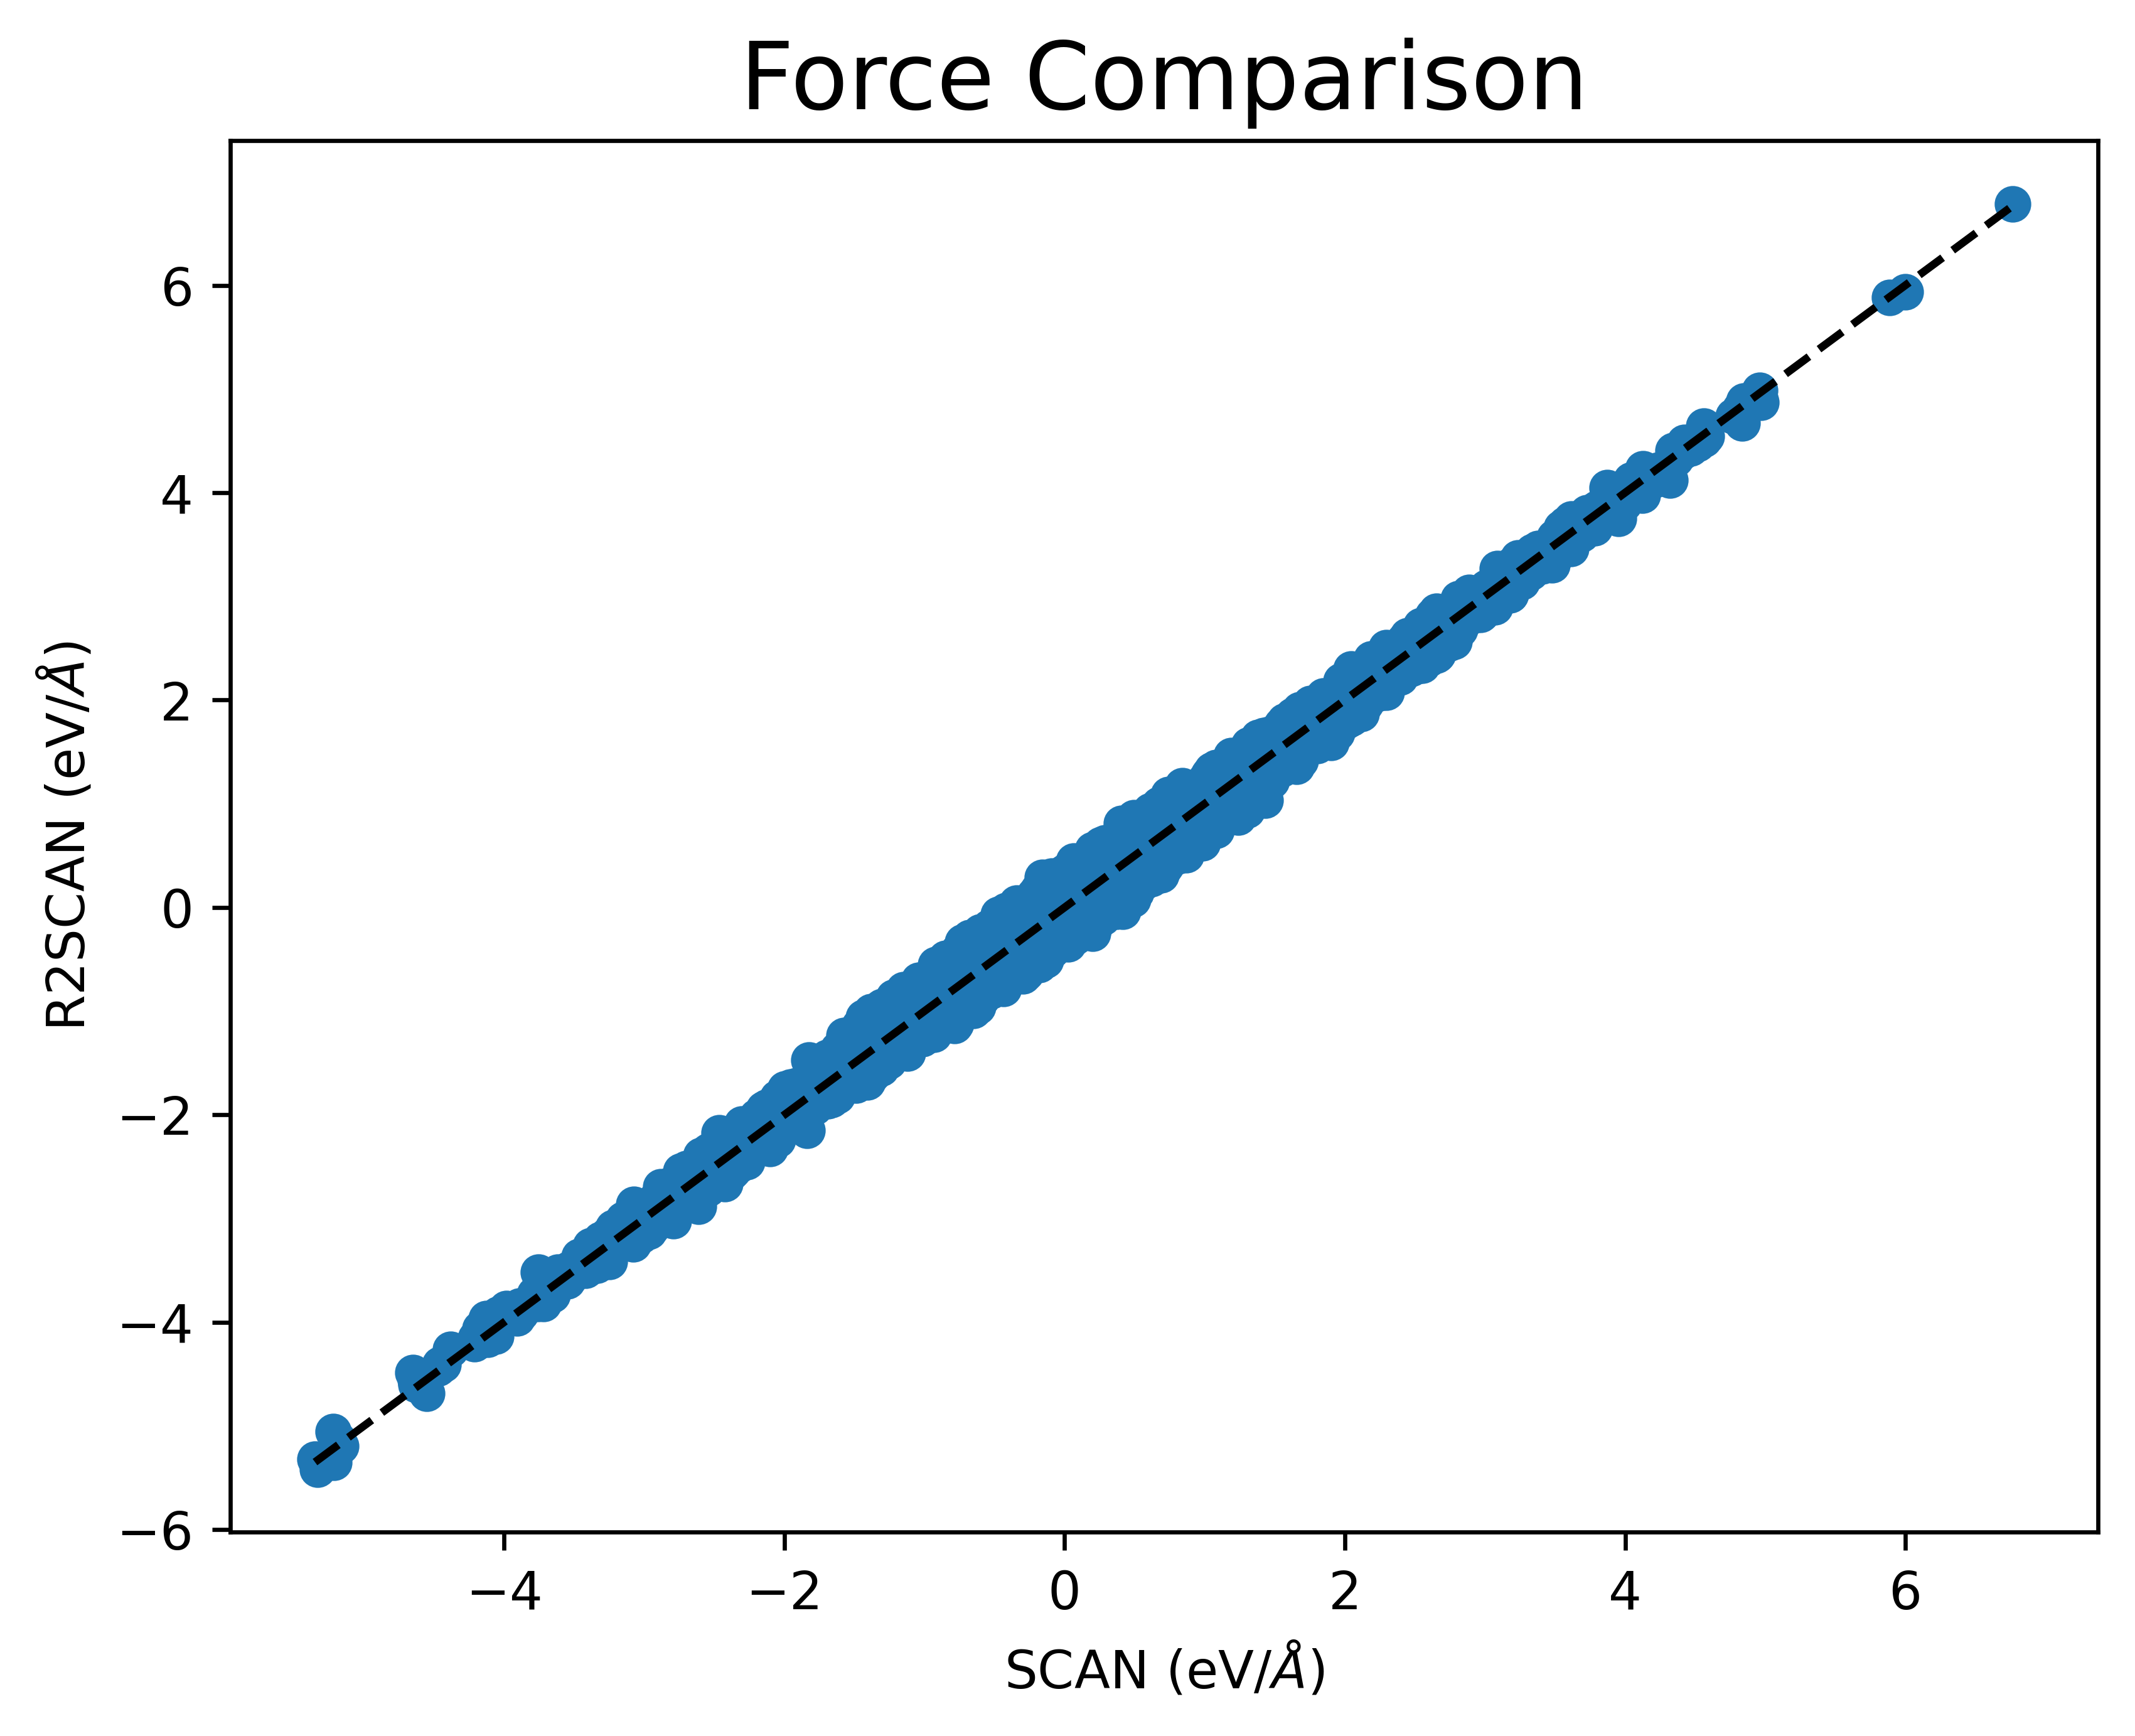
\includegraphics[width=0.9\textwidth]{images/scan_vs_r2scan/force_compare.png}
		\caption{Atomic Force Comparison}\label{fig:scan_r2scan_F}
	\end{subfigure}

	\caption{Correlation of  (a) relative total energy and (b) atomic force
		between 		the		SCAN and
		r$^2$SCAN functional. The relative total energy was shifted to
		the lowest energy of each corresponding functional. The
		diagonal line shows the
		perfect
		agreement between
		the two functionals.}\label{fig:scan_r2scan}
\end{figure}

\section{Neural Network Performance}
To assess the quality of deep NN models, model deviation was calculated for four identical models with different initialization parameters. For each new configuration explored during an MD run, these models generate an ensemble of predictions. The model deviation for each configuration is defined as the maximum standard deviation of the predicted atomic forces~\cite{zhang2019active,zeng2023deepmd}.  A small deviation indicates that the model has learned the given data; otherwise, it suggests that the configuration was not adequately covered, and the training data needs to be expanded. Note that only the first model was used as a many-body potential during the MD run to generate trajectories and pressures throughout the simulation. When the bulk-trained NNP was used as a potential for interfacial systems, the maximum deviation in forces showed significant error, as depicted in Figure~\ref{fig:dev_bulk}, indicating that the NNP models produced significantly different force values for a given trajectory. This outcome is expected since the bulk-trained NNP cannot capture features associated with surfaces. During training, the NNP models may have converged to different minimized loss functions. On the other hand, Figure~\ref{fig:dev_bulk_interface} shows that the error is greatly reduced when the bulk+interface-trained NNP was used in the simulation of interfacial systems.

\begin{figure}[tbhp]
	\centering
	\begin{subfigure}{0.48\textwidth}
		\centering

		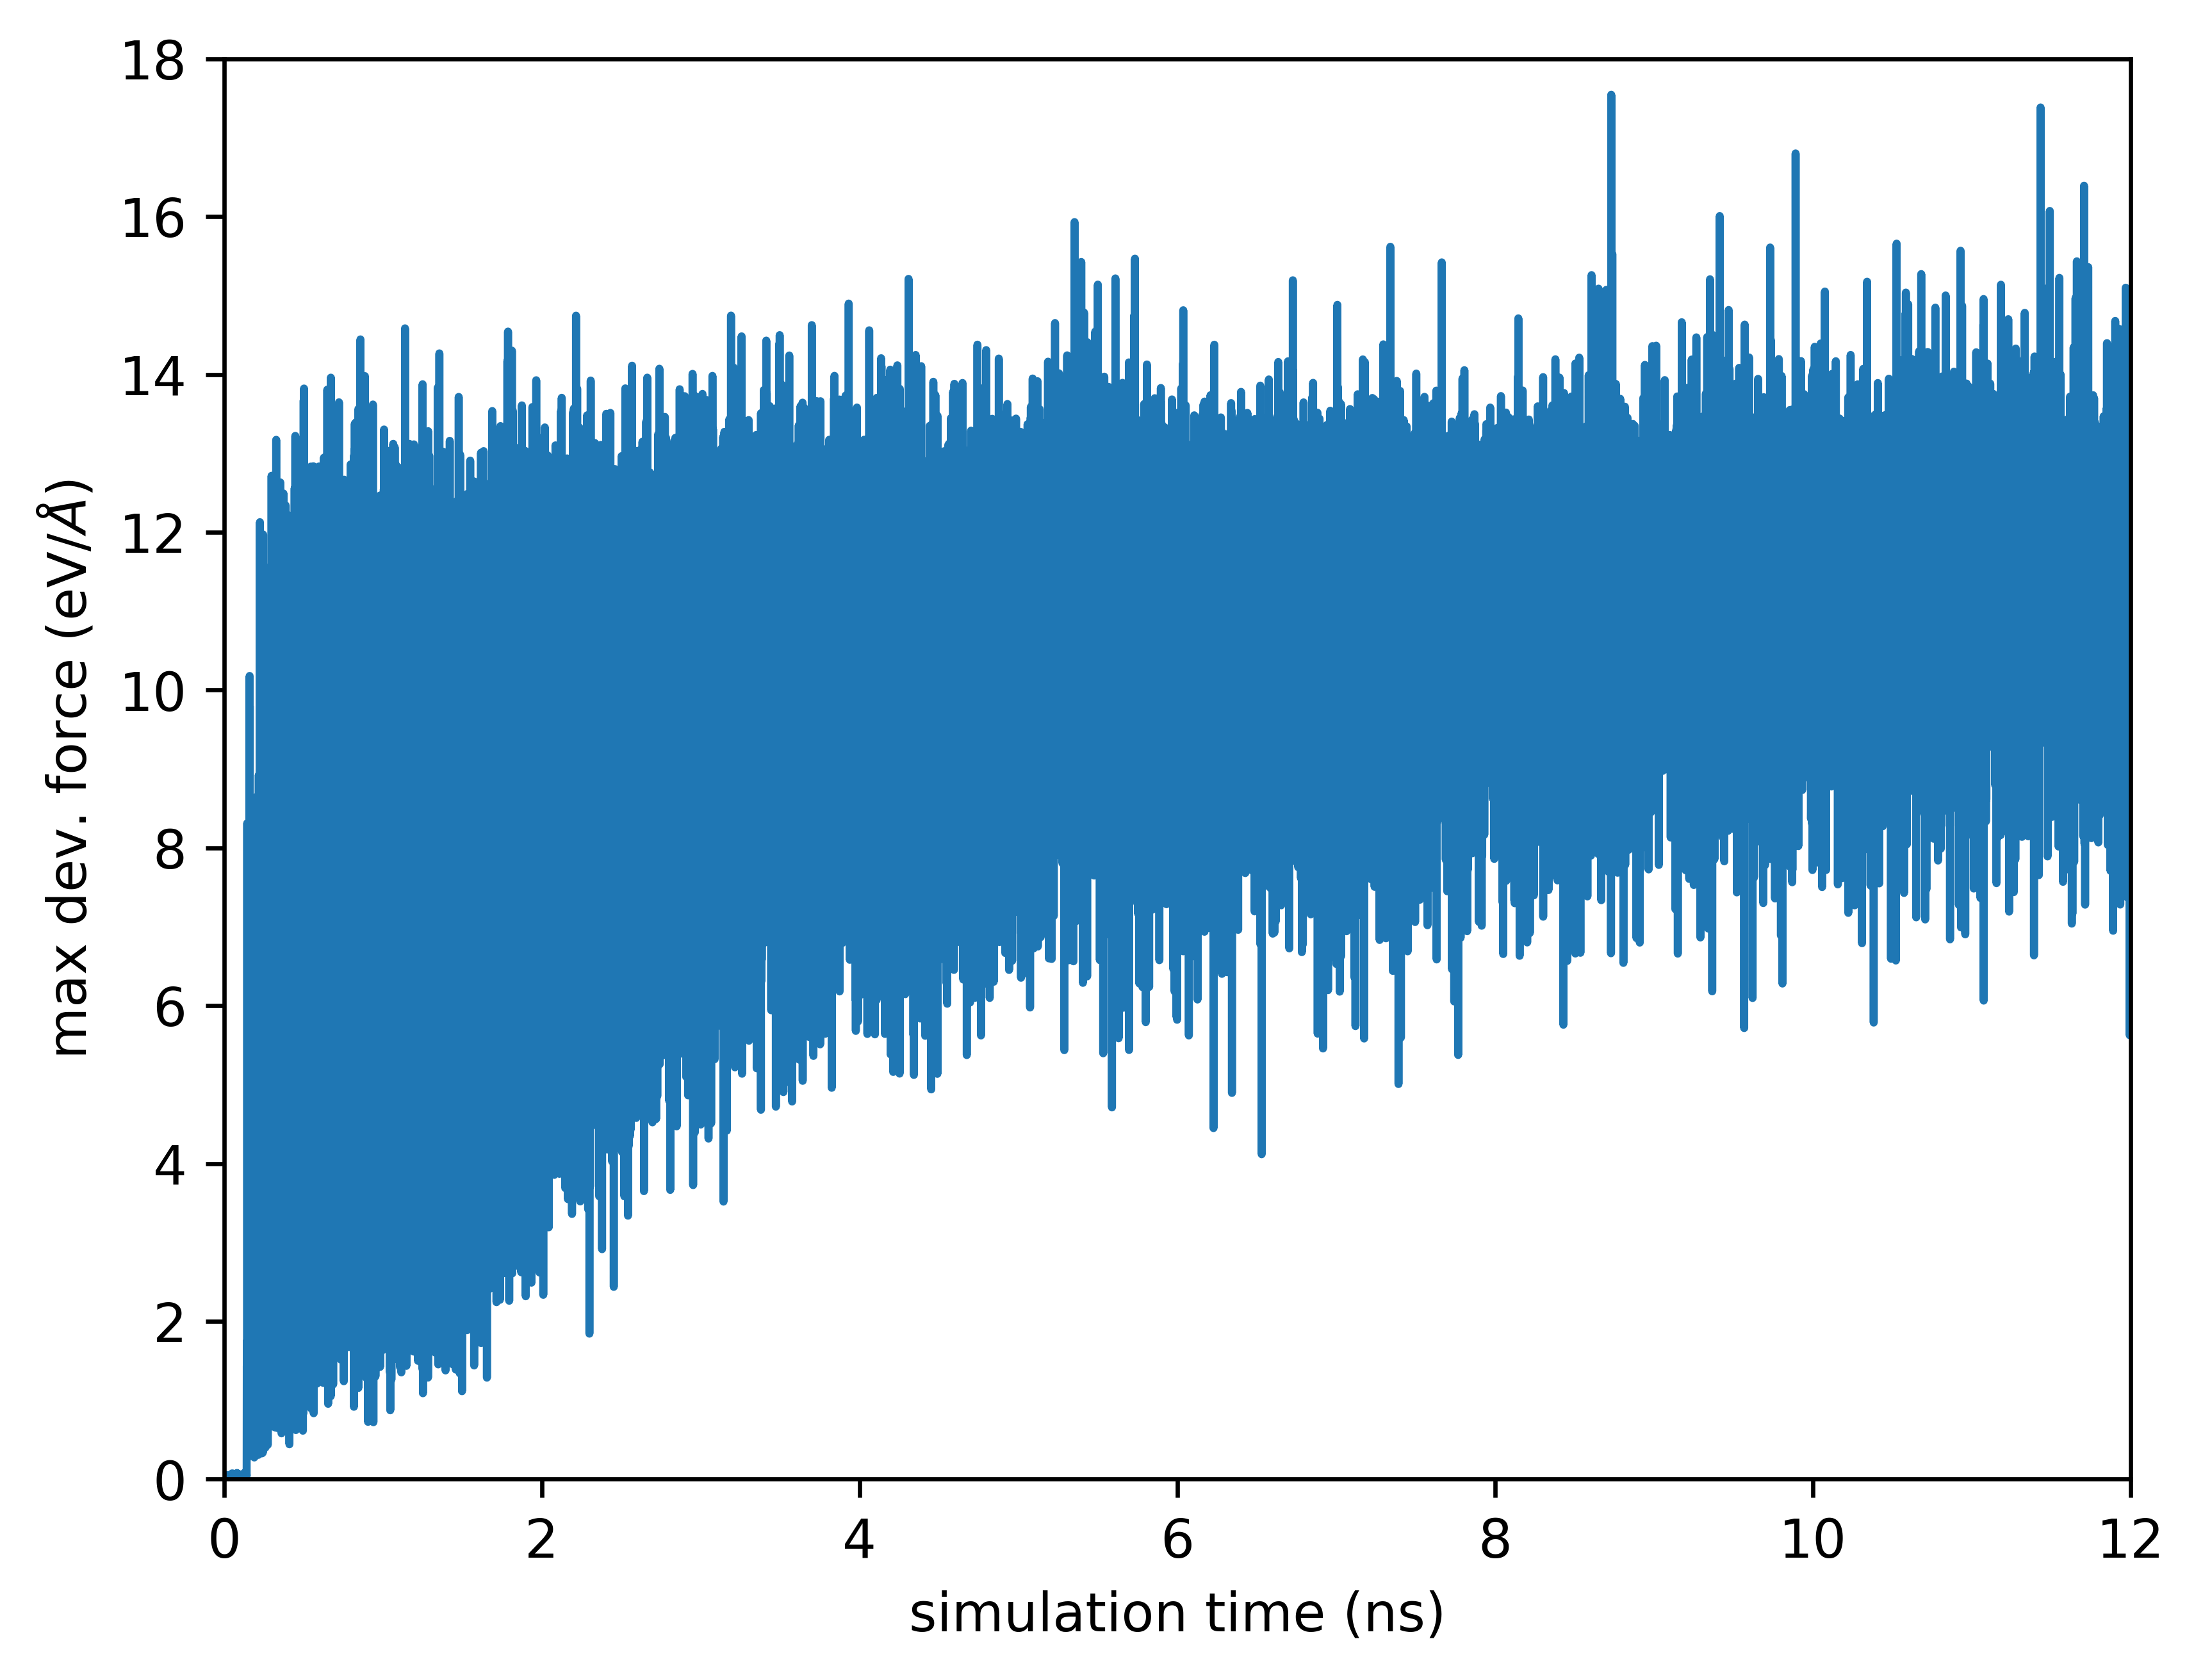
\includegraphics[width=0.9\textwidth]{images/deviation_bulk}
		\caption{Bulk-trained NNP}\label{fig:dev_bulk}
	\end{subfigure}
	\hfill
	\begin{subfigure}{0.48\textwidth}
		\centering

		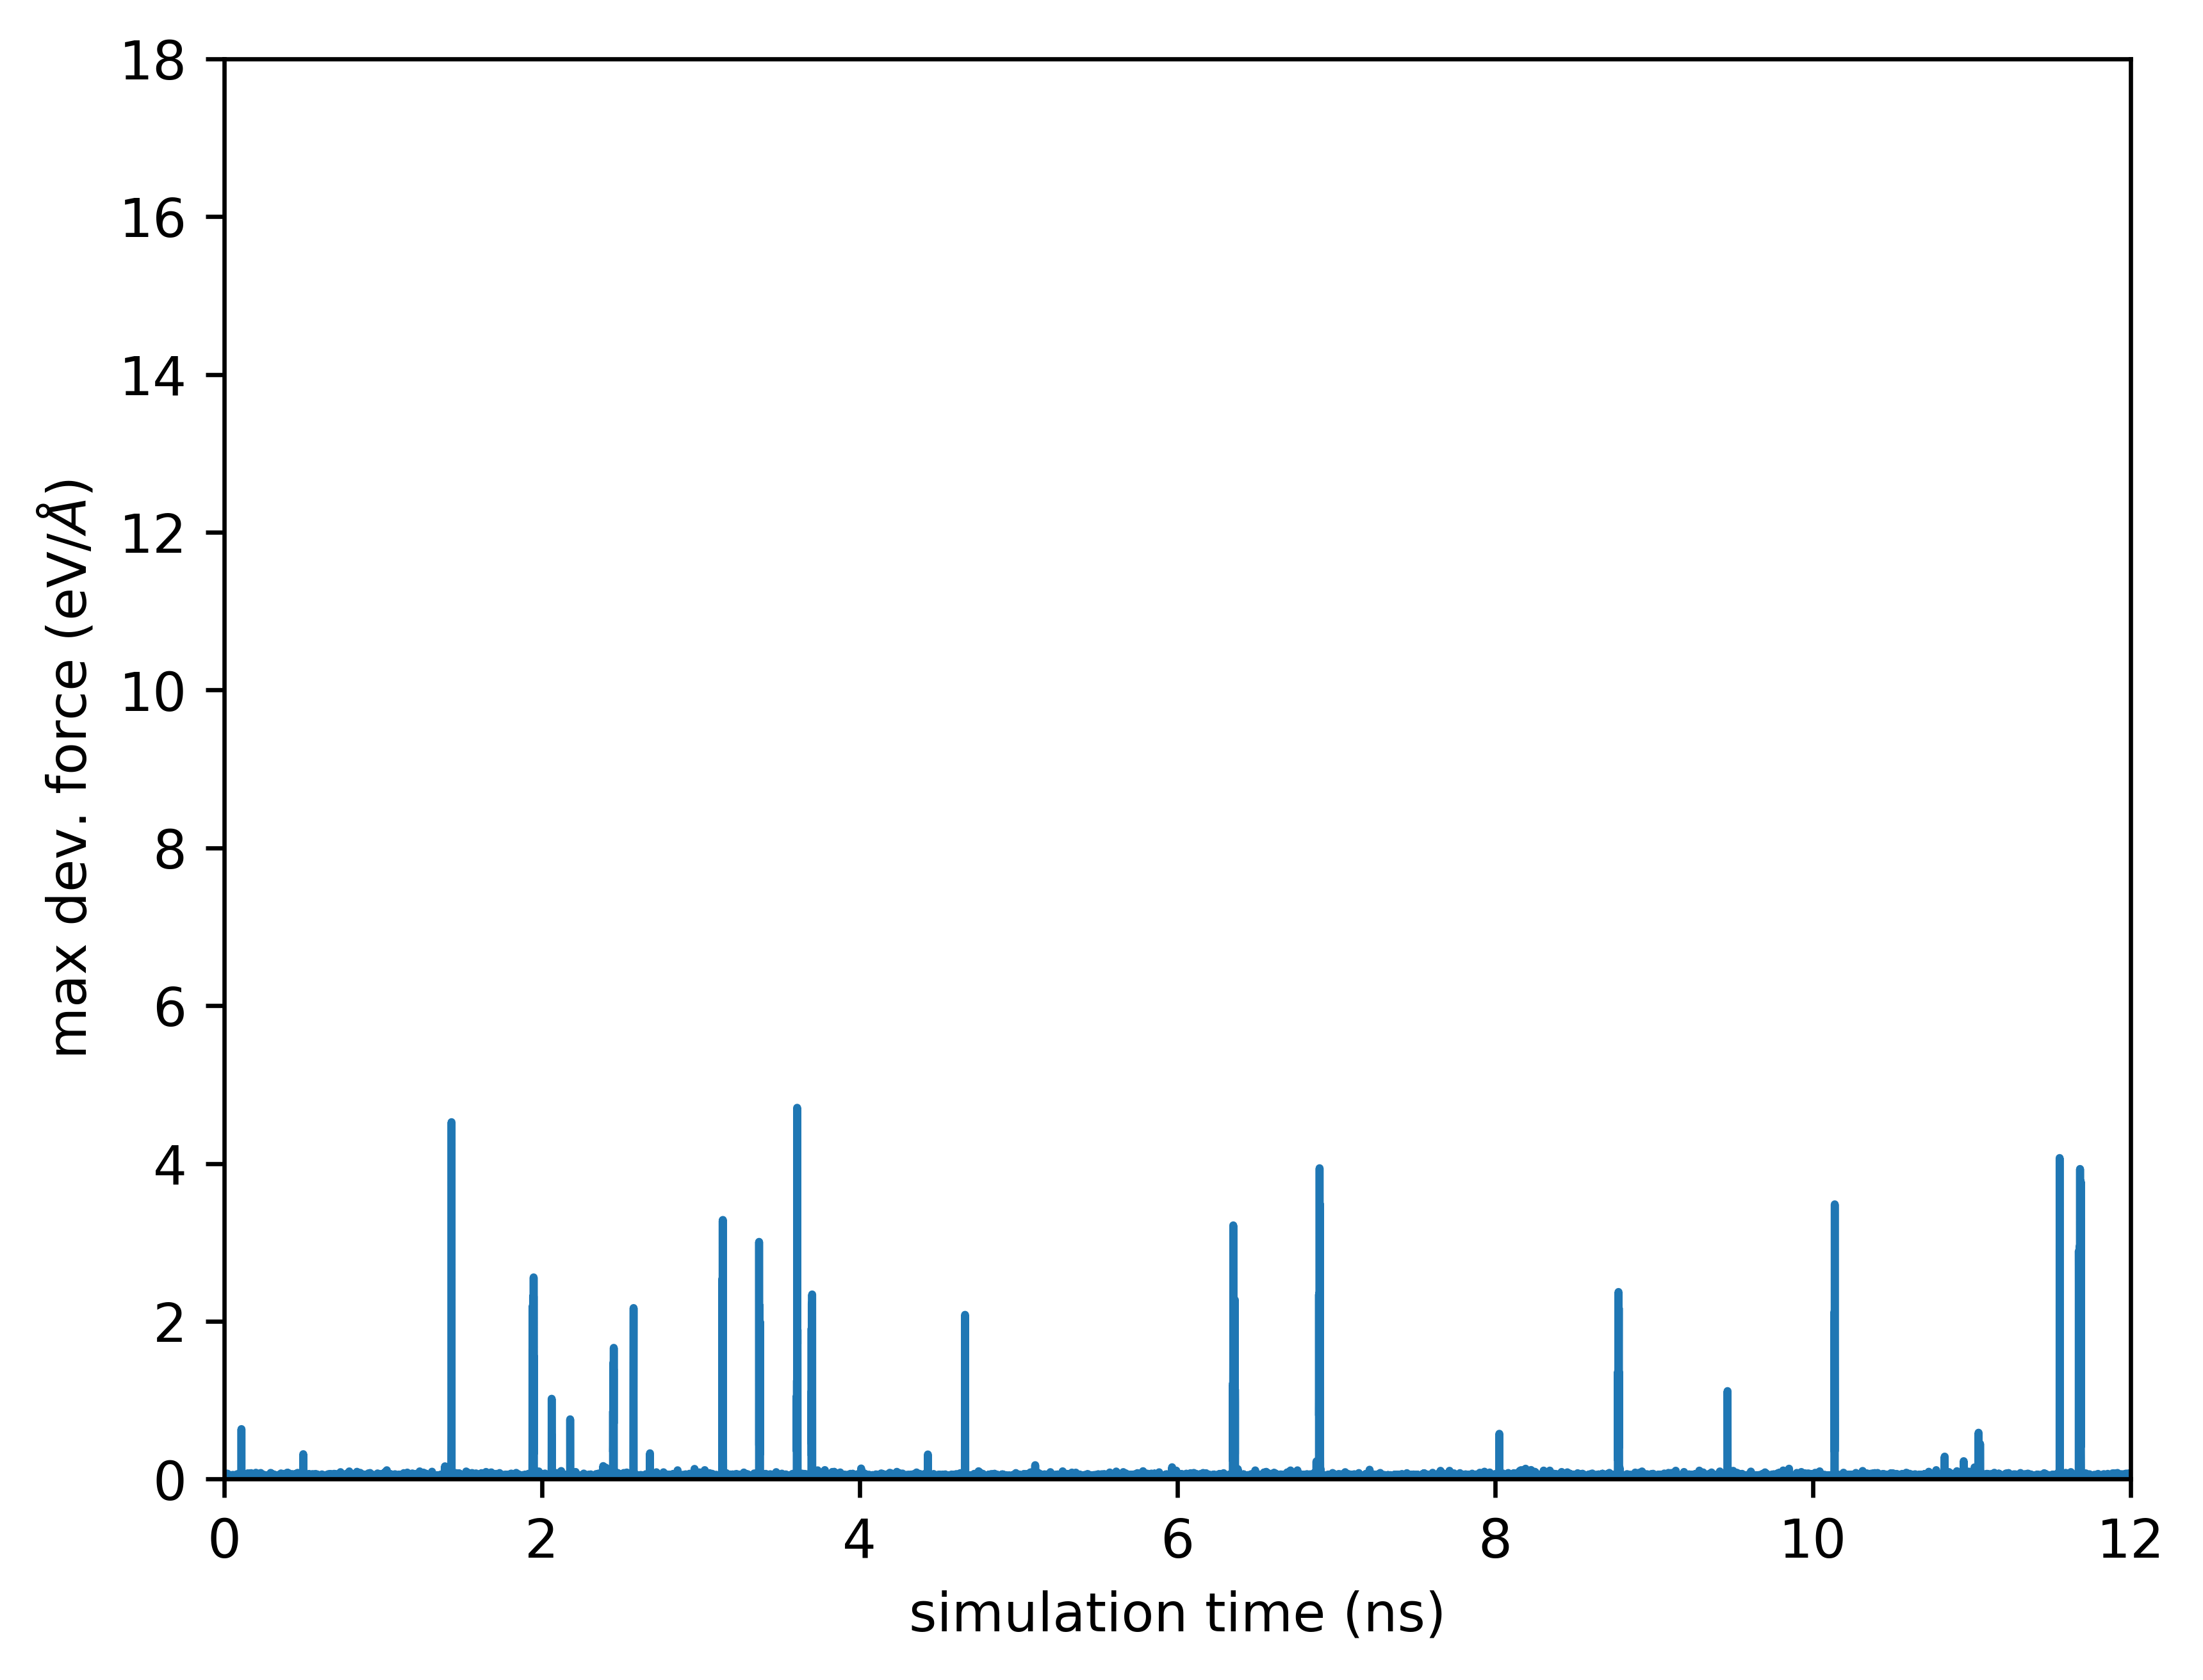
\includegraphics[width=0.9\textwidth]{images/deviation_bulk+interface}
		\caption{Bulk+Interface-trained NNP}\label{fig:dev_bulk_interface}
	\end{subfigure}

	\caption{Stability of (a) bulk-trained NNP and (b) bulk+interface
		trained NNP when used as many-body potential in MD simulation of
		interfacial
		systems. }\label{fig:model_dev}
\end{figure}

A test was conducted to evaluate the accuracy of the trained neural network potentials in predicting energy, force, and virial relative to DFT data for interfacial systems. Table~\ref{tab:train_perf} lists the mean absolute error (MAE) and root mean square error (RMSE) for the bulk-trained NNP and the bulk+interface-trained NNP. The results show that the error is lower when the NNP is trained to include both bulk and interface environments. This is expected, as the model was trained to explore both bulk and interface environments. Specifically, there is a 59\% and 14\% improvement in RMSE for energy per atom and force, respectively, with the bulk+interface NNP compared to the bulk NNP.

\begin{table}[tbhp!]
	\centering
	\caption{Performance of bulk-trained NNP and
		bulk+interface-trained NNP on bulk+interface validation
		dataset.}\label{tab:train_perf}
	\resizebox{0.7\columnwidth}{!}{%
		\begin{tabular}{@{}lcc@{}}
			\toprule
			                        & Bulk-trained NNP &
			Bulk+Interface-trained NNP
			\\
			\midrule
			Energy MAE (eV)         & \num{5.195E-01}  &
			\num{1.939E-01}
			\\
			Energy	 RMSE	(eV)         & \num{6.222E-01}  &
			\num{2.616E-01}
			\\
			Energy MAE/Natoms (eV)  & \num{9.019E-04}  &
			\num{3.366E-04}
			\\
			Energy	 RMSE/Natoms (eV) & \num{1.080E-03}  &
			\num{4.541E-04}
			\\
			Force  MAE	(eV/A)        & \num{4.164E-02}  &
			\num{3.613E-02}
			\\
			Force  RMSE (eV/A)      & \num{5.654E-02}  &
			\num{4.836E-02}
			\\
			Virial MAE (eV)         & \num{5.886E-01}  &
			\num{5.491E-01}
			\\
			Virial	 RMSE (eV)        & \num{7.924E-01}  &
			\num{7.256E-01}
			\\
			Virial MAE/Natoms (eV)  & \num{1.020E-03}  &
			\num{9.533E-04}
			\\
			Virial	 RMSE/Natoms (eV) & \num{1.380E-03}  &
			\num{1.260E-03}
			\\
			\bottomrule
		\end{tabular}%
	}
\end{table}

Alternatively, one can check the correlation between the deep NN predictions and the DFT data. Figure~\ref{fig:corr_E} shows the relative total energy points, with the DFT data on one axis and the predictions from the neural network on the other, for both the bulk-trained and bulk+interface-trained NNP models. Notably, it can be seen that the predicted energies for the bulk-trained NNP are mostly underestimated, leading to higher test errors, as shown in Table~\ref{tab:train_perf}. On the other hand, the forces are in good agreement for both types of NNP models, as shown in Figure~\ref{fig:corr_F}.


\begin{figure}[tbhp!]
	\centering
	\begin{subfigure}{0.47\textwidth}
		\centering

		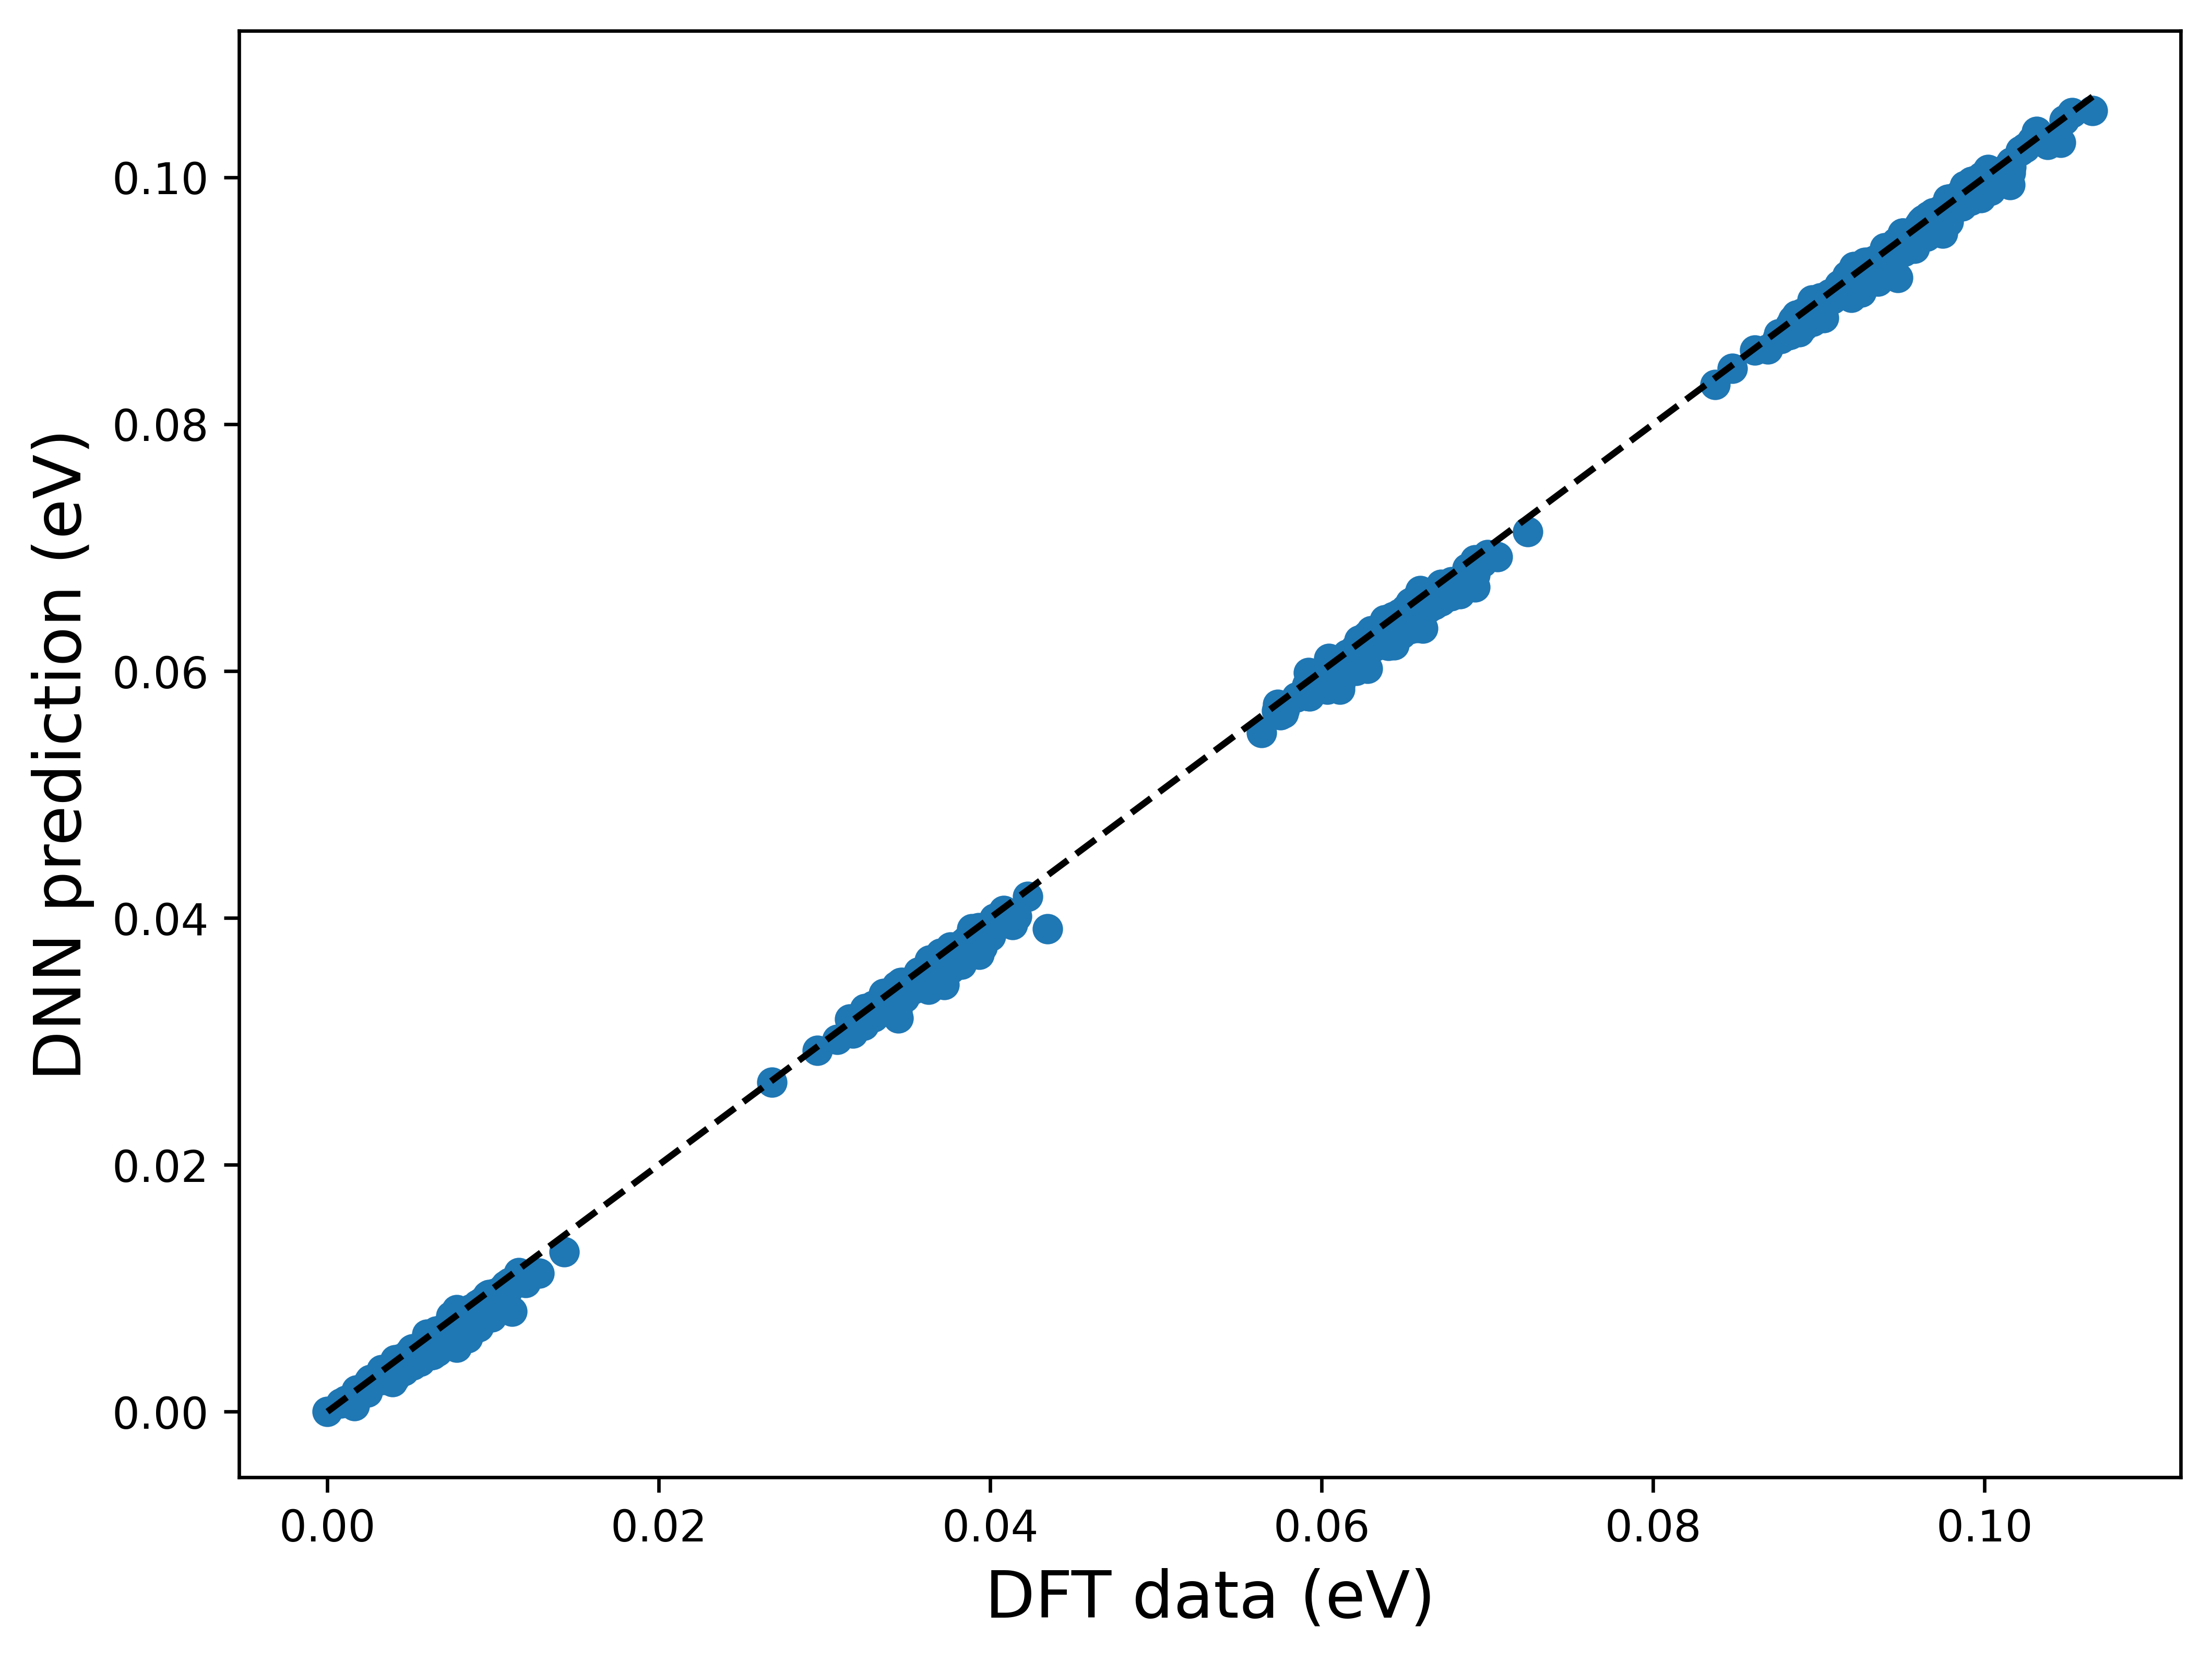
\includegraphics[width=0.9\textwidth]{images/bulk_NN_on_interface/2_e_peratom.png}
		\caption{Bulk-trained NNP}\label{fig:corr_bulk_NN_E}
	\end{subfigure}
	\hfill
	\begin{subfigure}{0.47\textwidth}
		\centering

		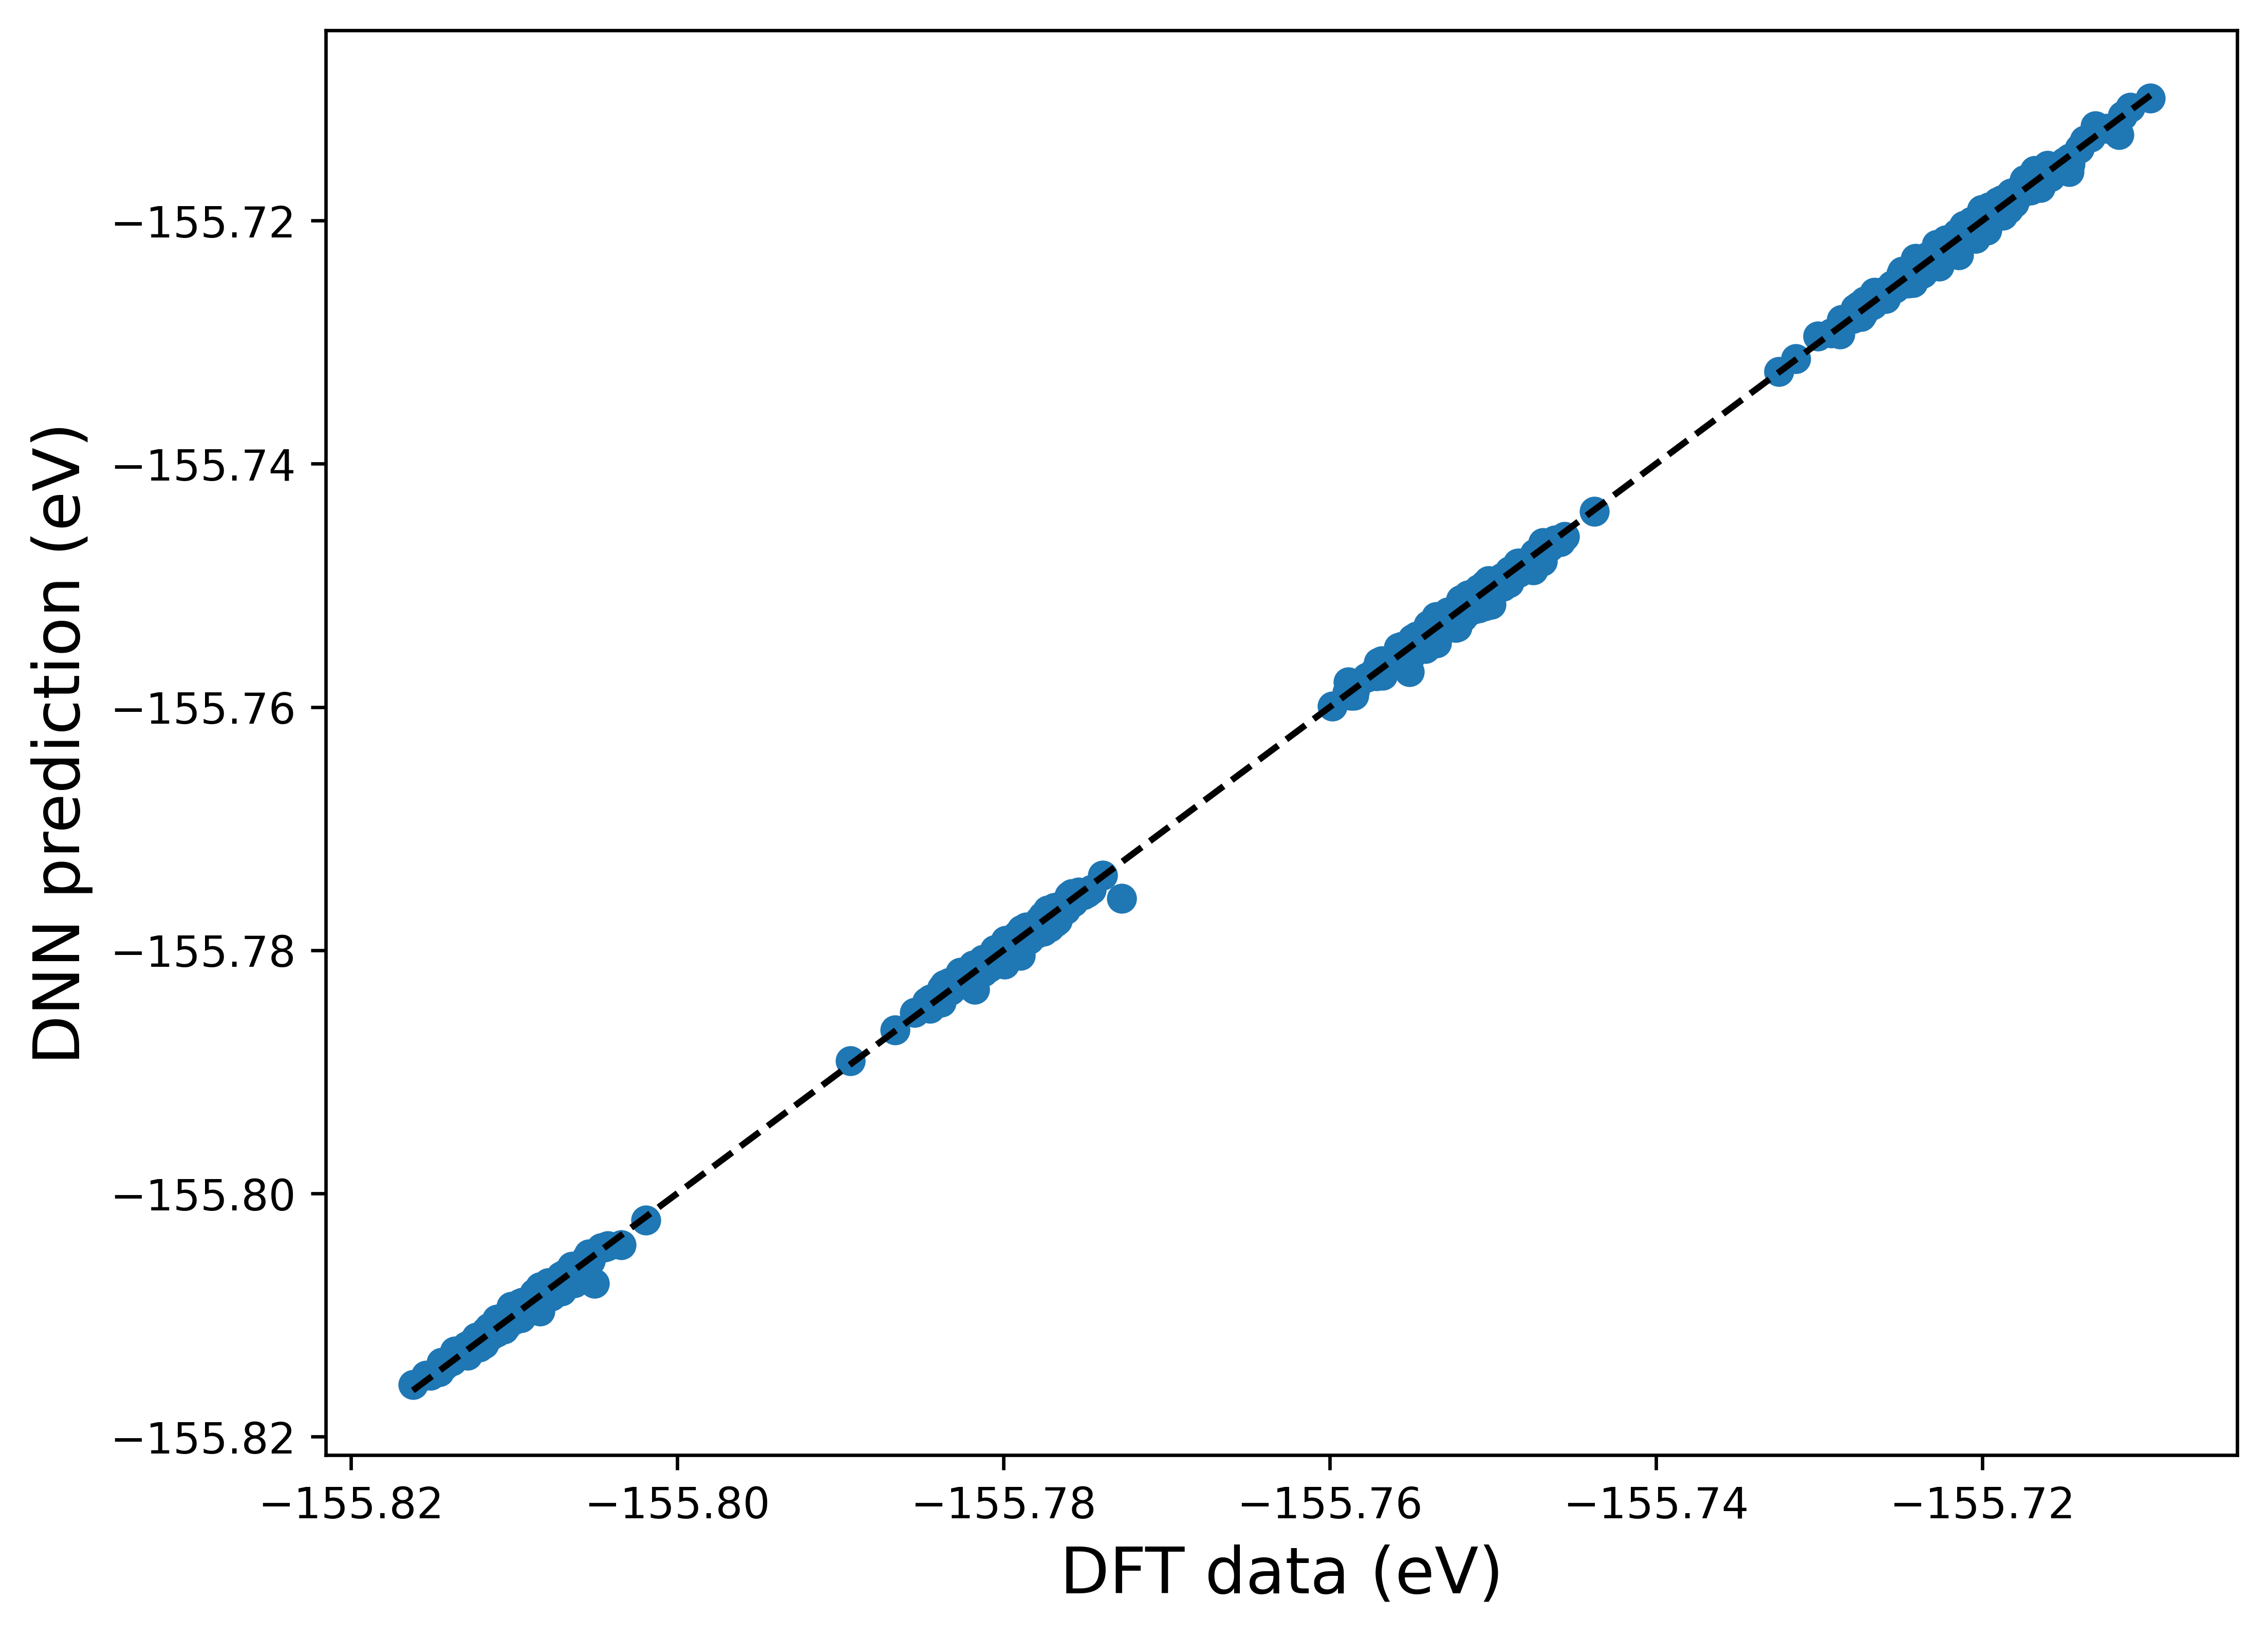
\includegraphics[width=0.9\textwidth]{images/bulk+interface_NN_on_interface/2_e_peratom.png}
		\caption{Bulk+Interface-trained NNP}\label{fig:corr_bulk+interface_NN_E}
	\end{subfigure}
	\caption{Relative total energy correlation between deep NN prediction data with
		the DFT data
		for a
		(a) bulk-trained NNP model and (b) bulk+interface-trained NNP
		model. The relative total energy was shifted to the lowest energy of each corresponding data. The diagonal line shows the perfect agreement between the two
		data.}\label{fig:corr_E}
\end{figure}

\clearpage

\begin{figure}[tbhp!]
	\centering
	\begin{subfigure}{0.47\textwidth}
		\centering

		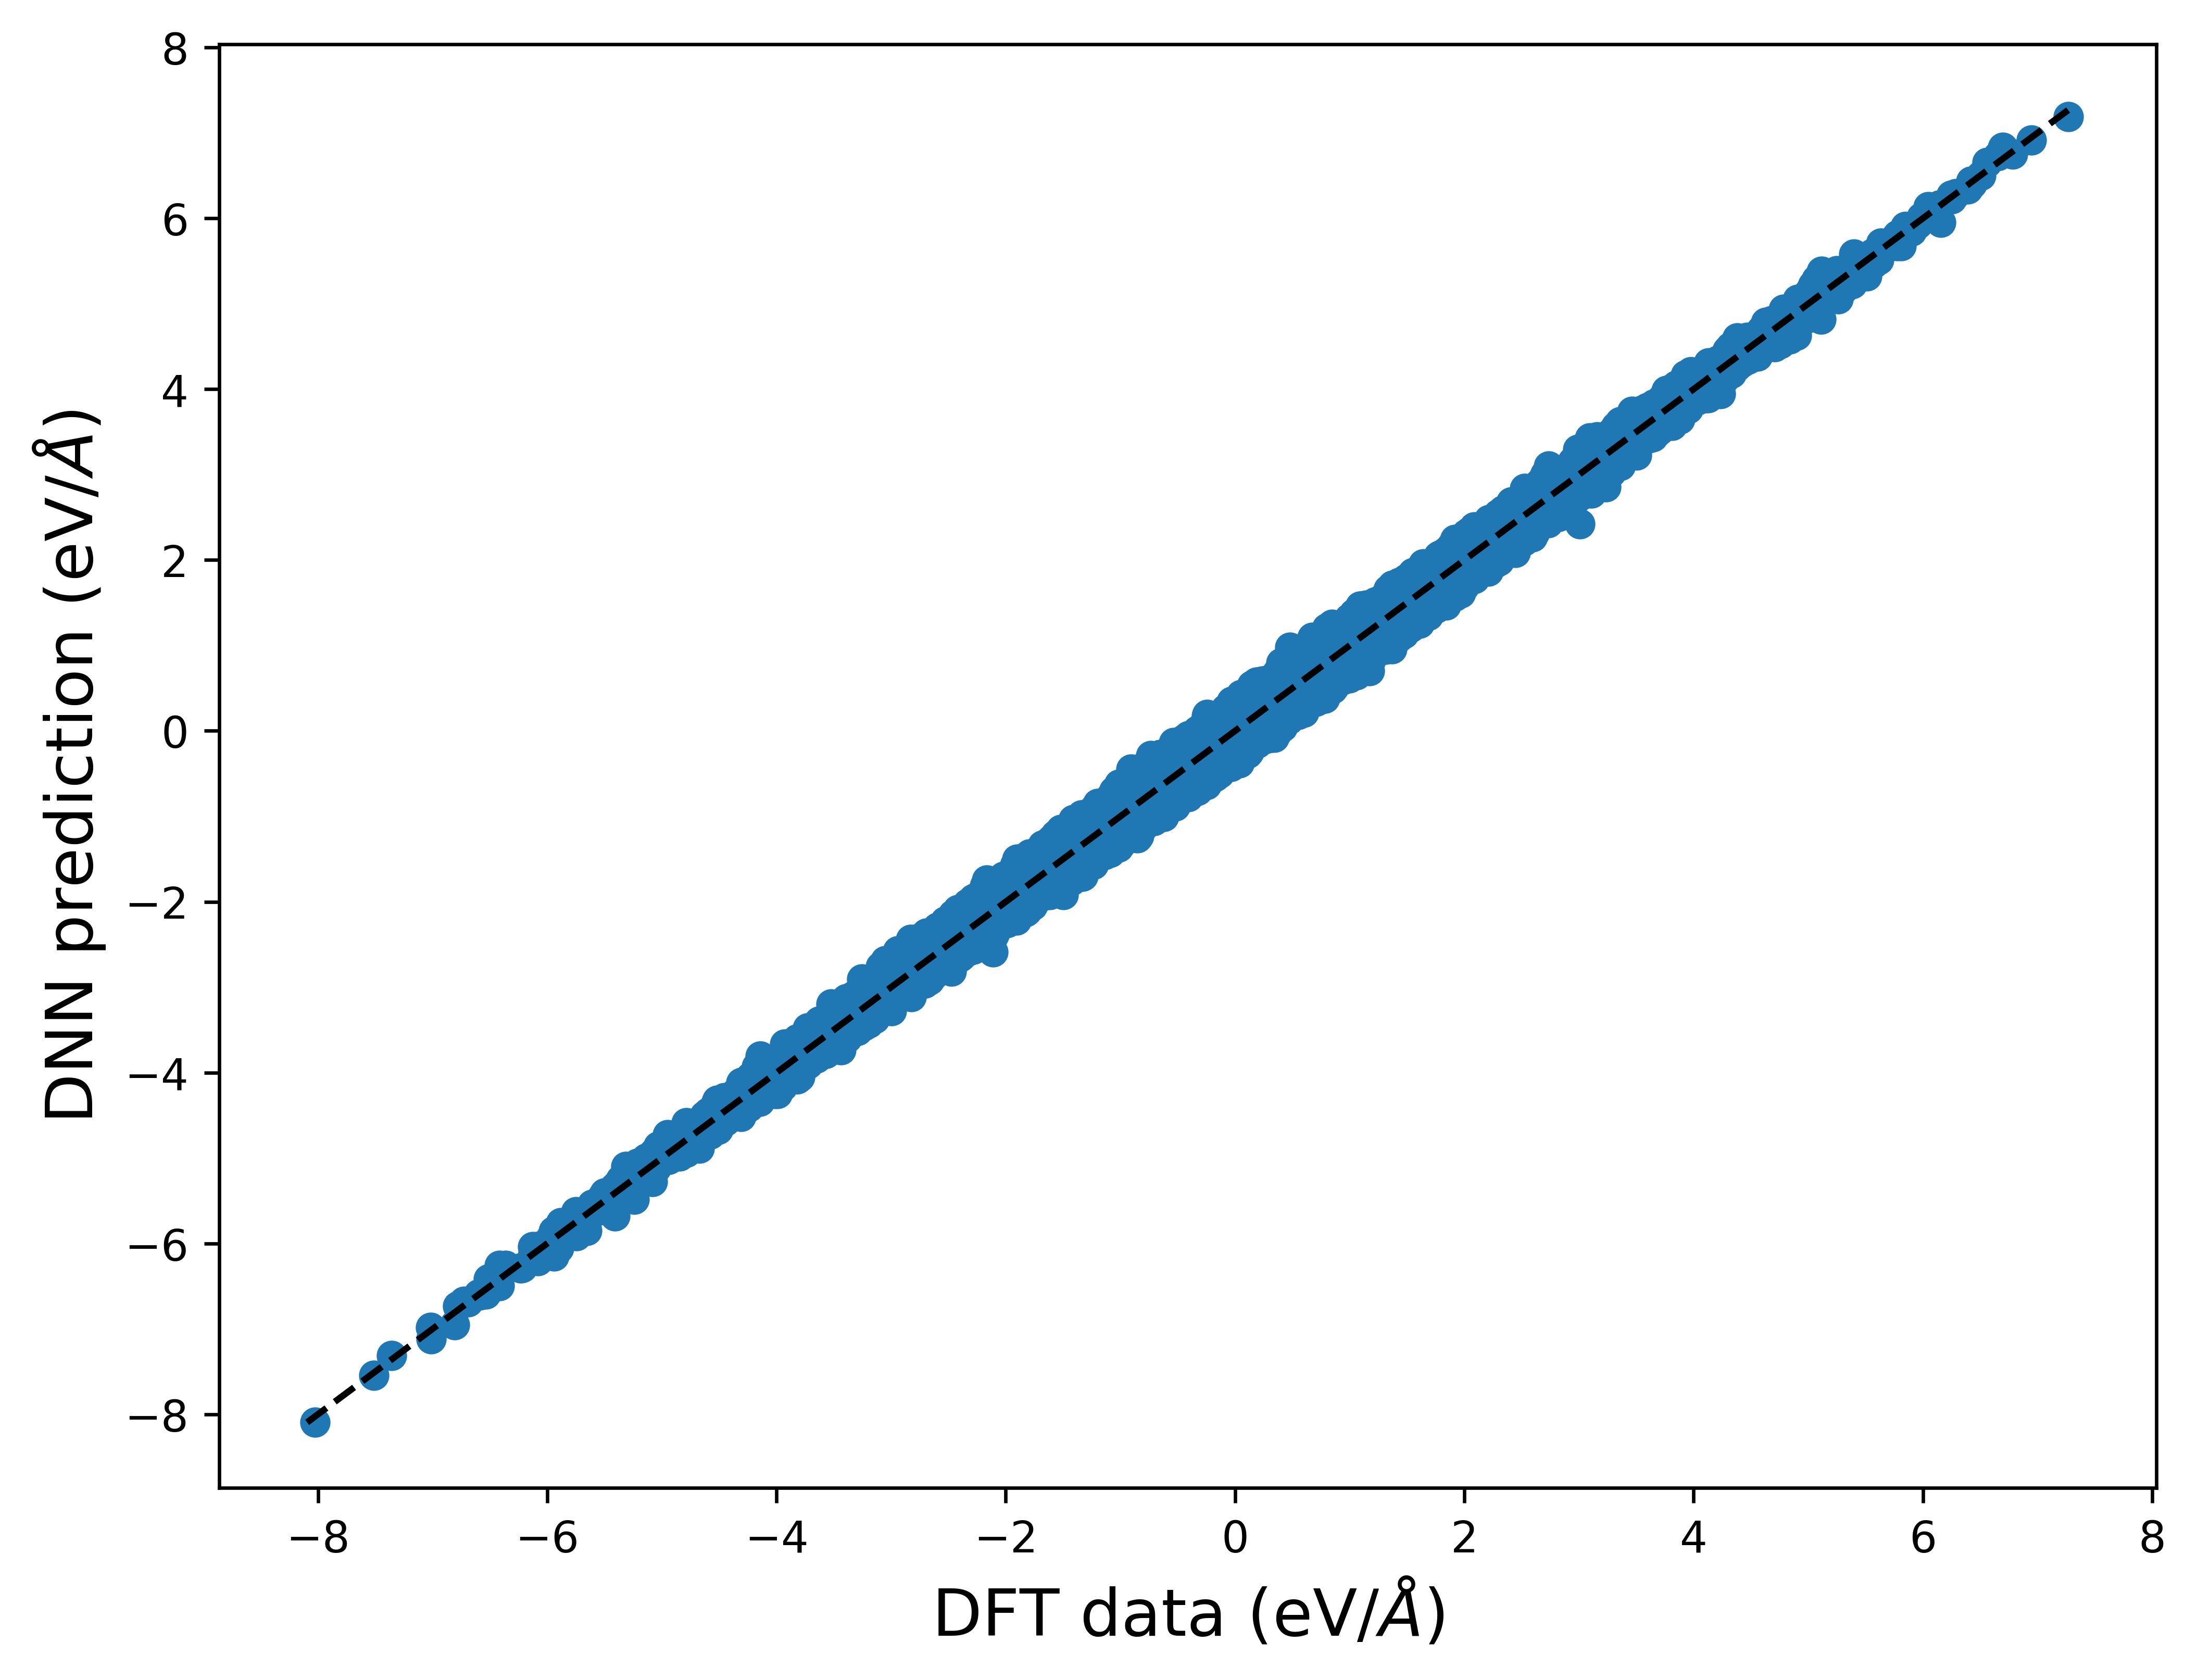
\includegraphics[width=0.9\textwidth]{images/bulk_NN_on_interface/2_force.png}
		\caption{Bulk-trained NNP}\label{fig:corr_bulk_NN_F}
	\end{subfigure}
	\hfill
	\begin{subfigure}{0.47\textwidth}
		\centering

		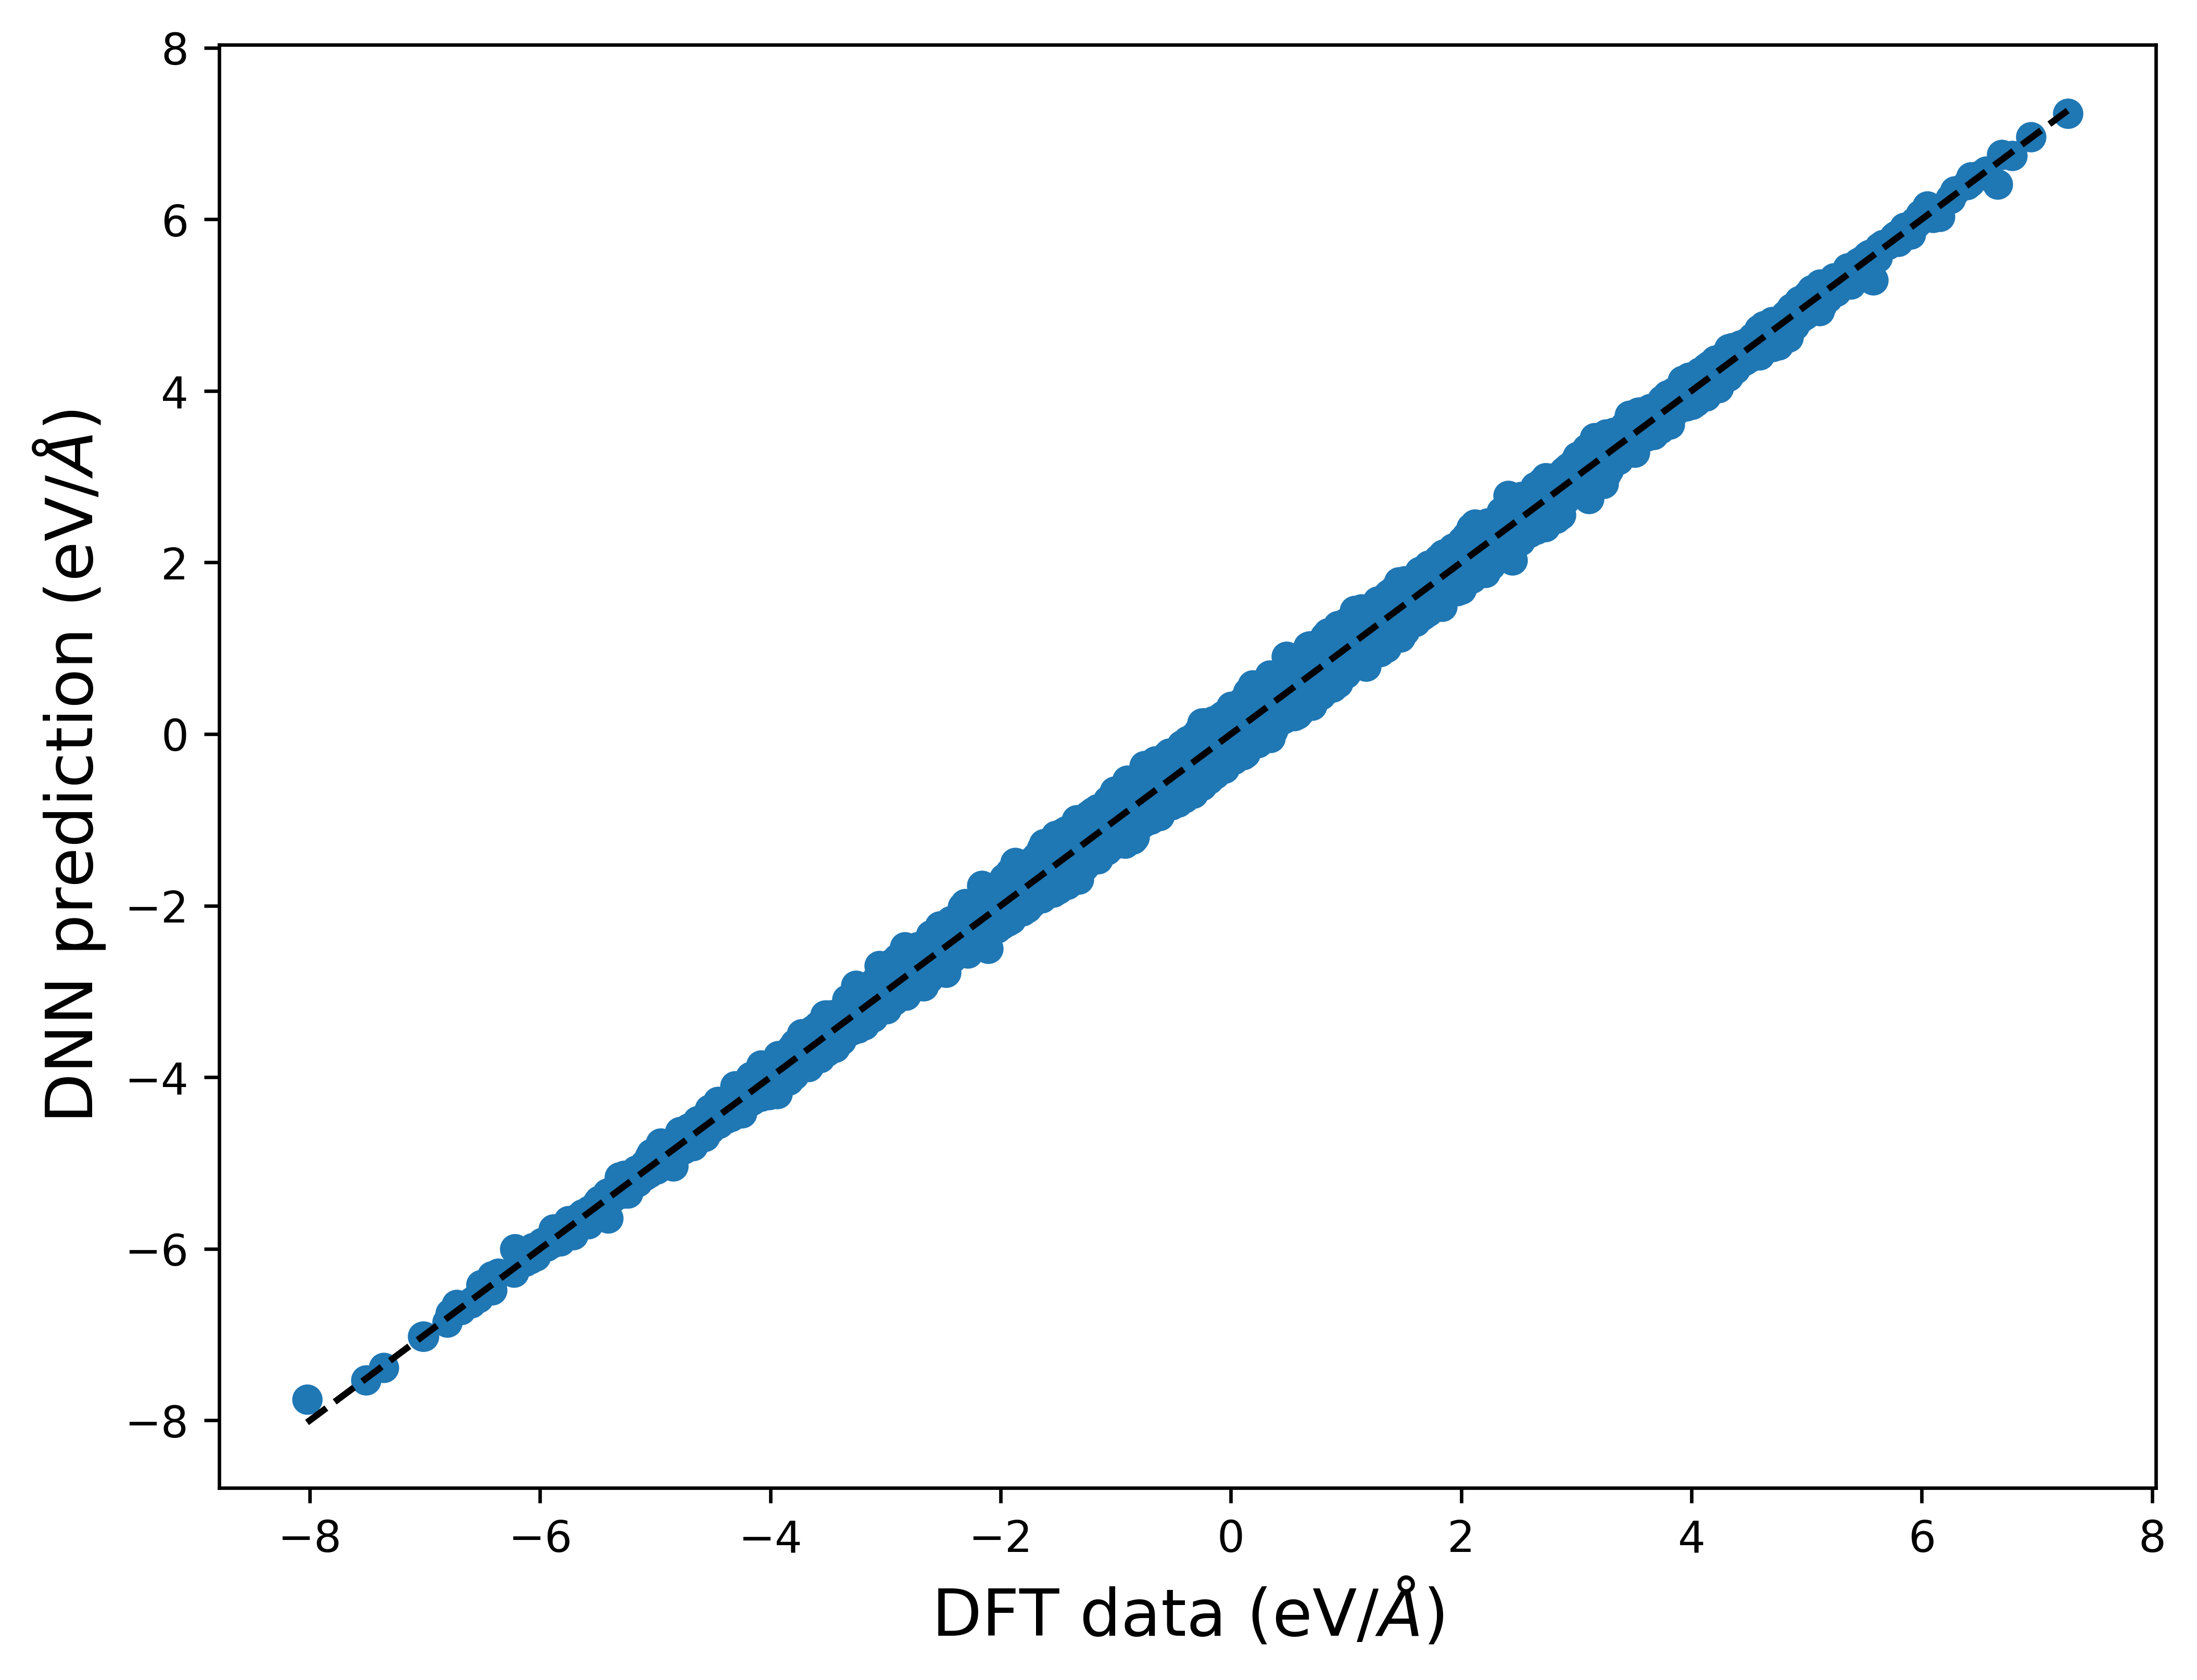
\includegraphics[width=0.9\textwidth]{images/bulk+interface_NN_on_interface/2_force.png}
		\caption{Bulk+Interface-trained NNP}\label{fig:corr_bulk+interface_NN_F}
	\end{subfigure}
	\caption{Atomic force correlation between deep NN prediction data with
		the DFT data
		for a
		(a) bulk-trained NNP model and (b) bulk+interface-trained NNP
		model. The
		diagonal line shows the perfect agreement between the two
		data.}\label{fig:corr_F}
\end{figure}

\section{Mass Density}

For all MD simulations, the temperature was set to the ambient temperature of 300 K. To account for the shift in the melting temperature of ice when using the SCAN functional, a +30 K adjustment was applied, so 330 K represents the new ambient temperature~\cite{piaggi2021phase}.

Figure~\ref{fig:density} shows the mass density of 192 water molecules at 330 K for different deep neural network models. The results of fitting the mass density profile using Eq.\ref{eq:fit_dens} are listed in Table\ref{tab:density_fit}. The NNP model trained on bulk environments has a bulk density of 0.974 \unit{g/cm^3}, which is underestimated by 2.61\% from the experimental value of 1.00 \unit{g/cm^3}. In contrast, the reference model from the work of Sanchez-Burgos et al.~\cite{sanchez2023deep} has a bulk density of 1.031 \unit{g/cm^3}, which is overestimated by 3.09\%. Note that the reference model was trained on bulk environments only and used the SCAN functional. Meanwhile, the NNP model trained on both bulk and interface systems has a bulk density of 0.994 \unit{g/cm^3}, which is the most accurate among the models. Additionally, the bulk+interface-trained NNP accurately describes the bulk region, as indicated by the smaller fluctuations in density values compared to the other models. Interfacial thickness was also quantified, with the bulk+interface-trained NNP having the smallest thickness of 1.360 \unit{\angstrom} among the models, followed by the reference NNP with a thickness of 1.410 \unit{\angstrom}, and then the bulk-trained NNP with a thickness of 1.546 \unit{\angstrom}. Experimental measurements of interfacial thickness are of the order of 3.2 \unit{\angstrom}~\cite{braslau1985surface}, about twice as large as the values obtained from the NNP models. This large discrepancy has been attributed to the suppression of capillary waves due to the finite size of the simulation cell~\cite{matsumoto1988study}.


\begin{figure}[tbhp!]
	\centering
	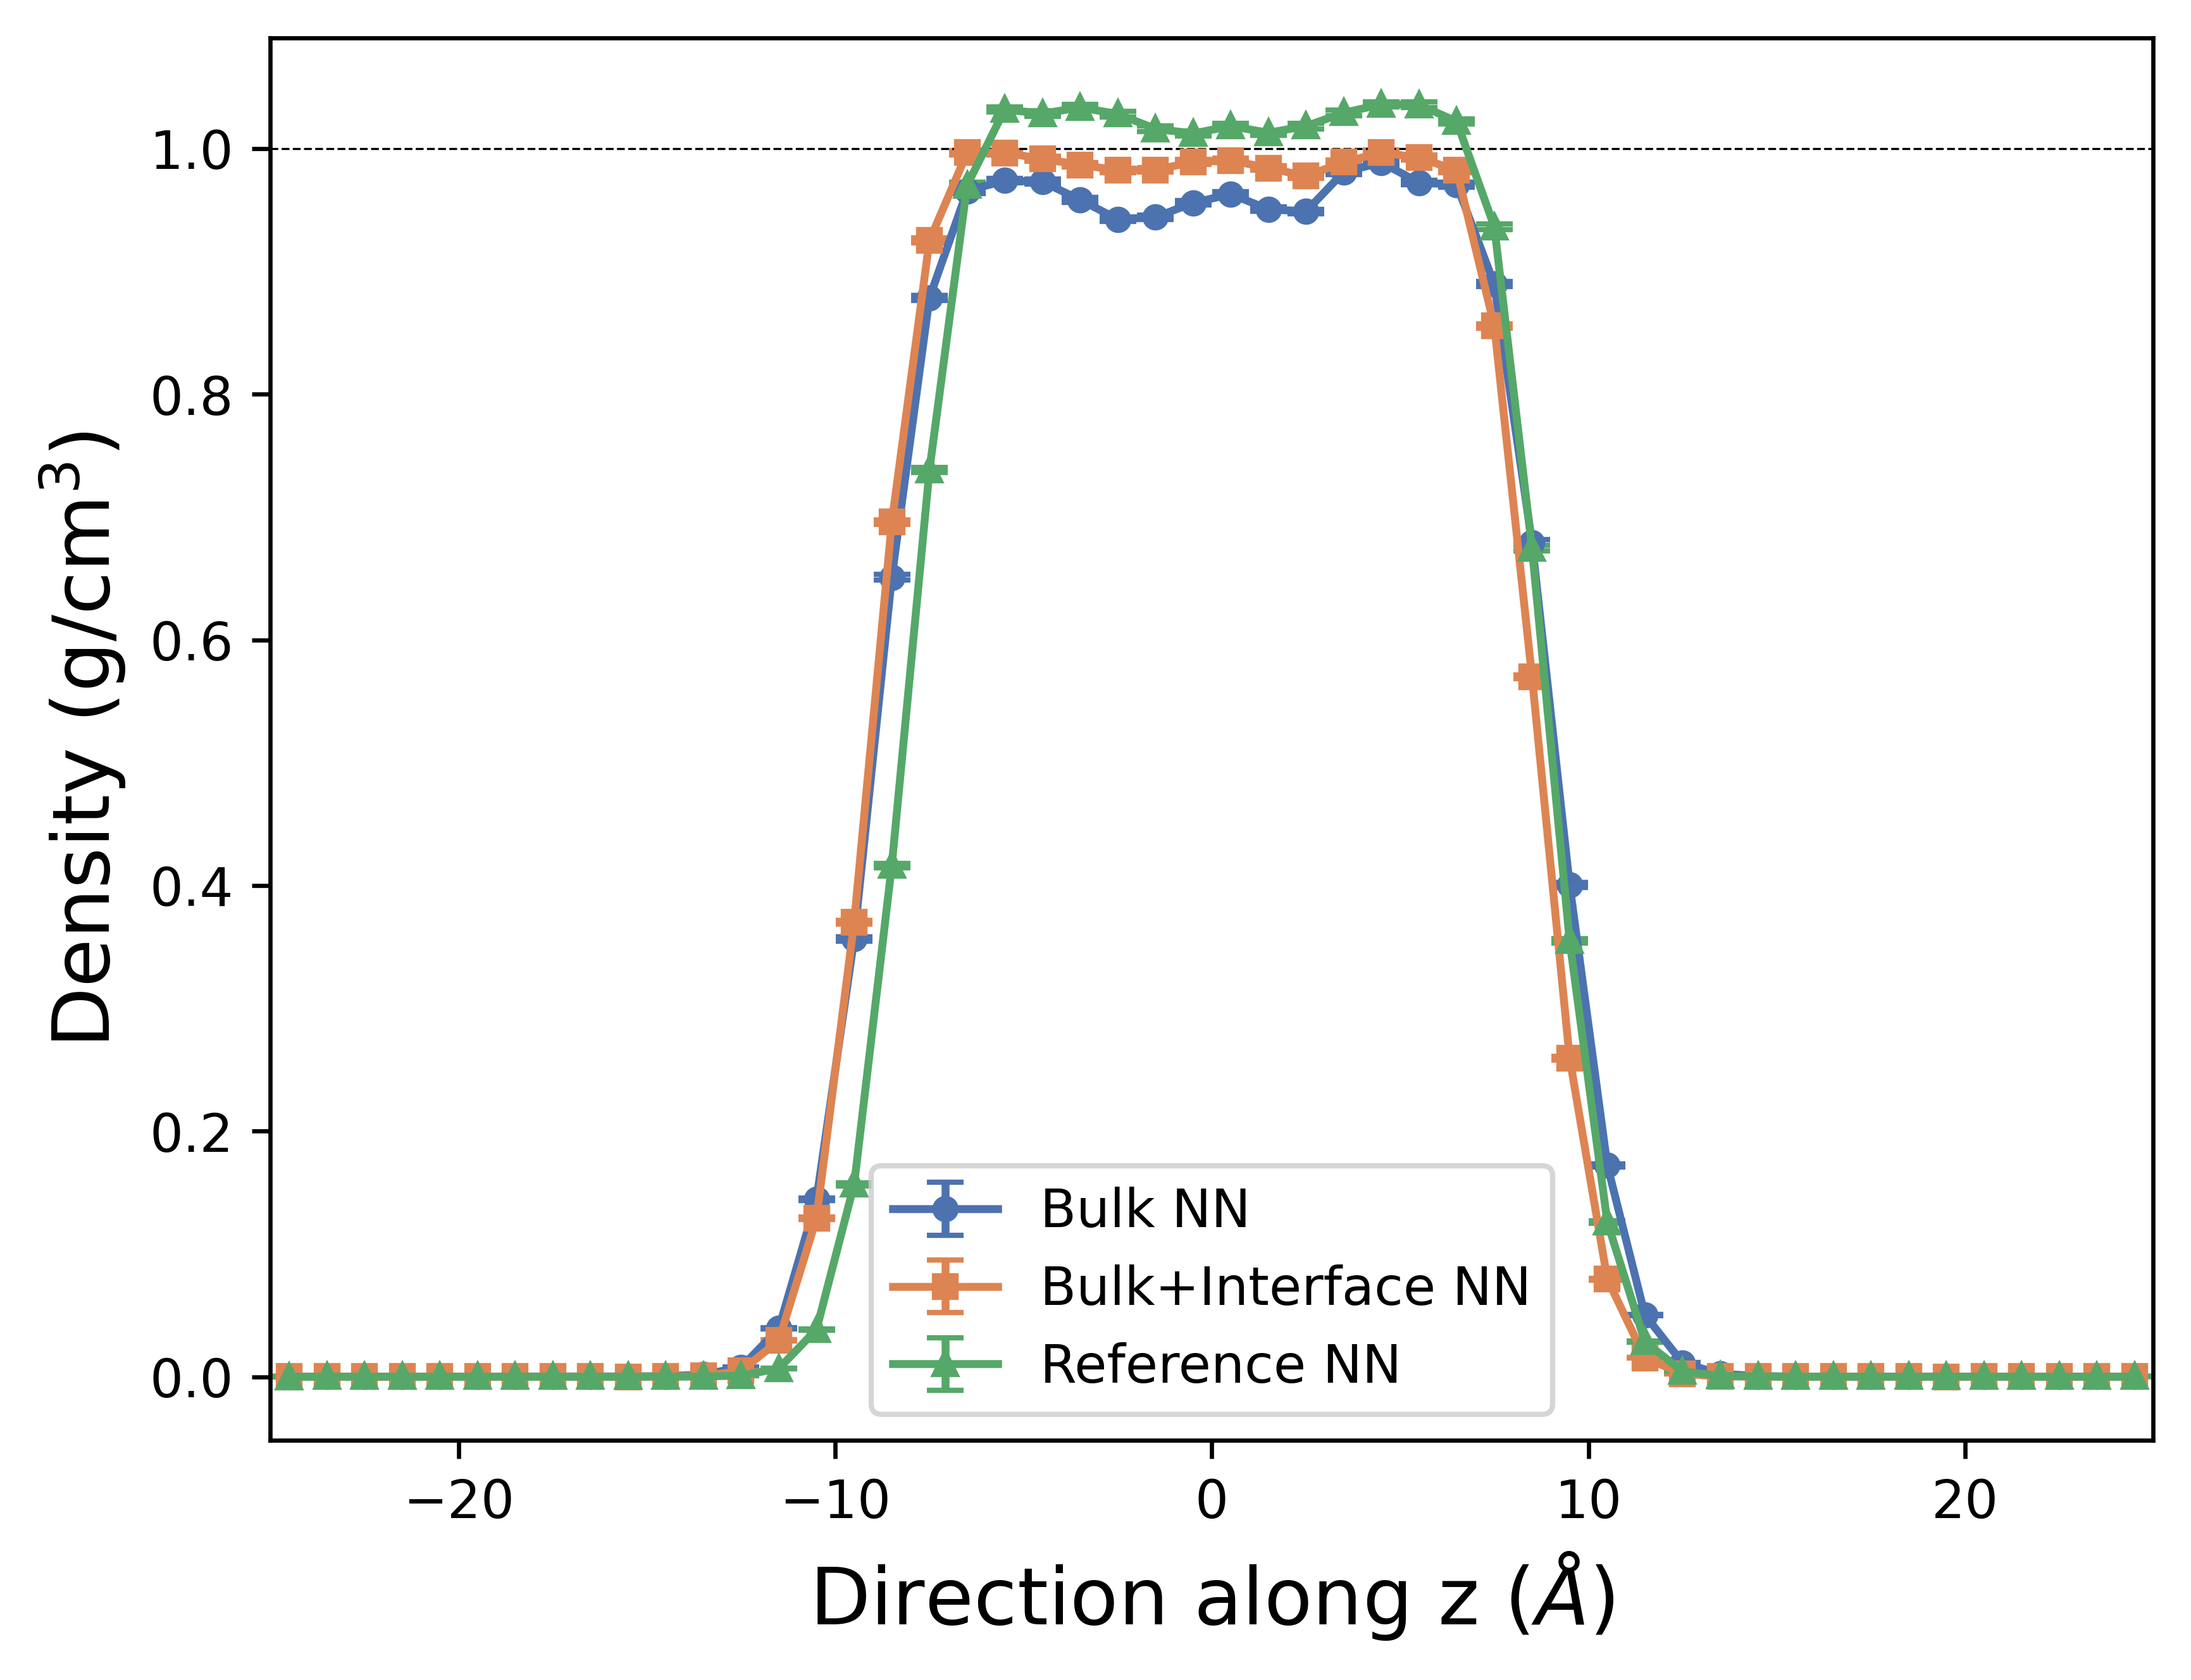
\includegraphics[width=0.65\linewidth]{images/density_330.png}
	\caption{Mass Density Profile at 330 K for different deep neural
		network
		models. The reference model is based on trained model of
		Sanchez-Burgos et
		al.~\cite{sanchez2023deep}. }\label{fig:density}
\end{figure}


\section{Surface Tension}
Surface tension was calculated according to the formula in Eq.~\eqref{eq:surf_tens}. For a bulk system, this equation is expected to yield zero since pressure is isotropic in all directions. However, for systems with interfaces, symmetry is broken along the direction normal to the surface, resulting in a nonzero surface tension.

Figure~\ref{fig:surf_tens} shows the plot of surface tension as a function of temperature for different NNP models. The bulk-only trained NNP model produces poor results, with significantly underestimated values that begin to plateau above 400 K. In contrast, the bulk+interface-trained NNP model shows a much better improvement in surface tension predictions, particularly at higher temperatures. This result supports the idea that surface defects play a role in accurately predicting interfacial properties such as surface tension. The reference model is more accurate, even though it was trained only on bulk environments. However, the reference model was trained on a very large dataset that includes both ice and liquid phases and covers a vast thermodynamic range up to 2000 K and 50 GPa~\cite{zhang2021phase}. In comparison, our bulk+interface-trained NNP model was trained over a thermodynamic range up to 600 K and 1 GPa, yet still provides comparable accuracy to the reference model.


\begin{figure}[h!]
	\centering
	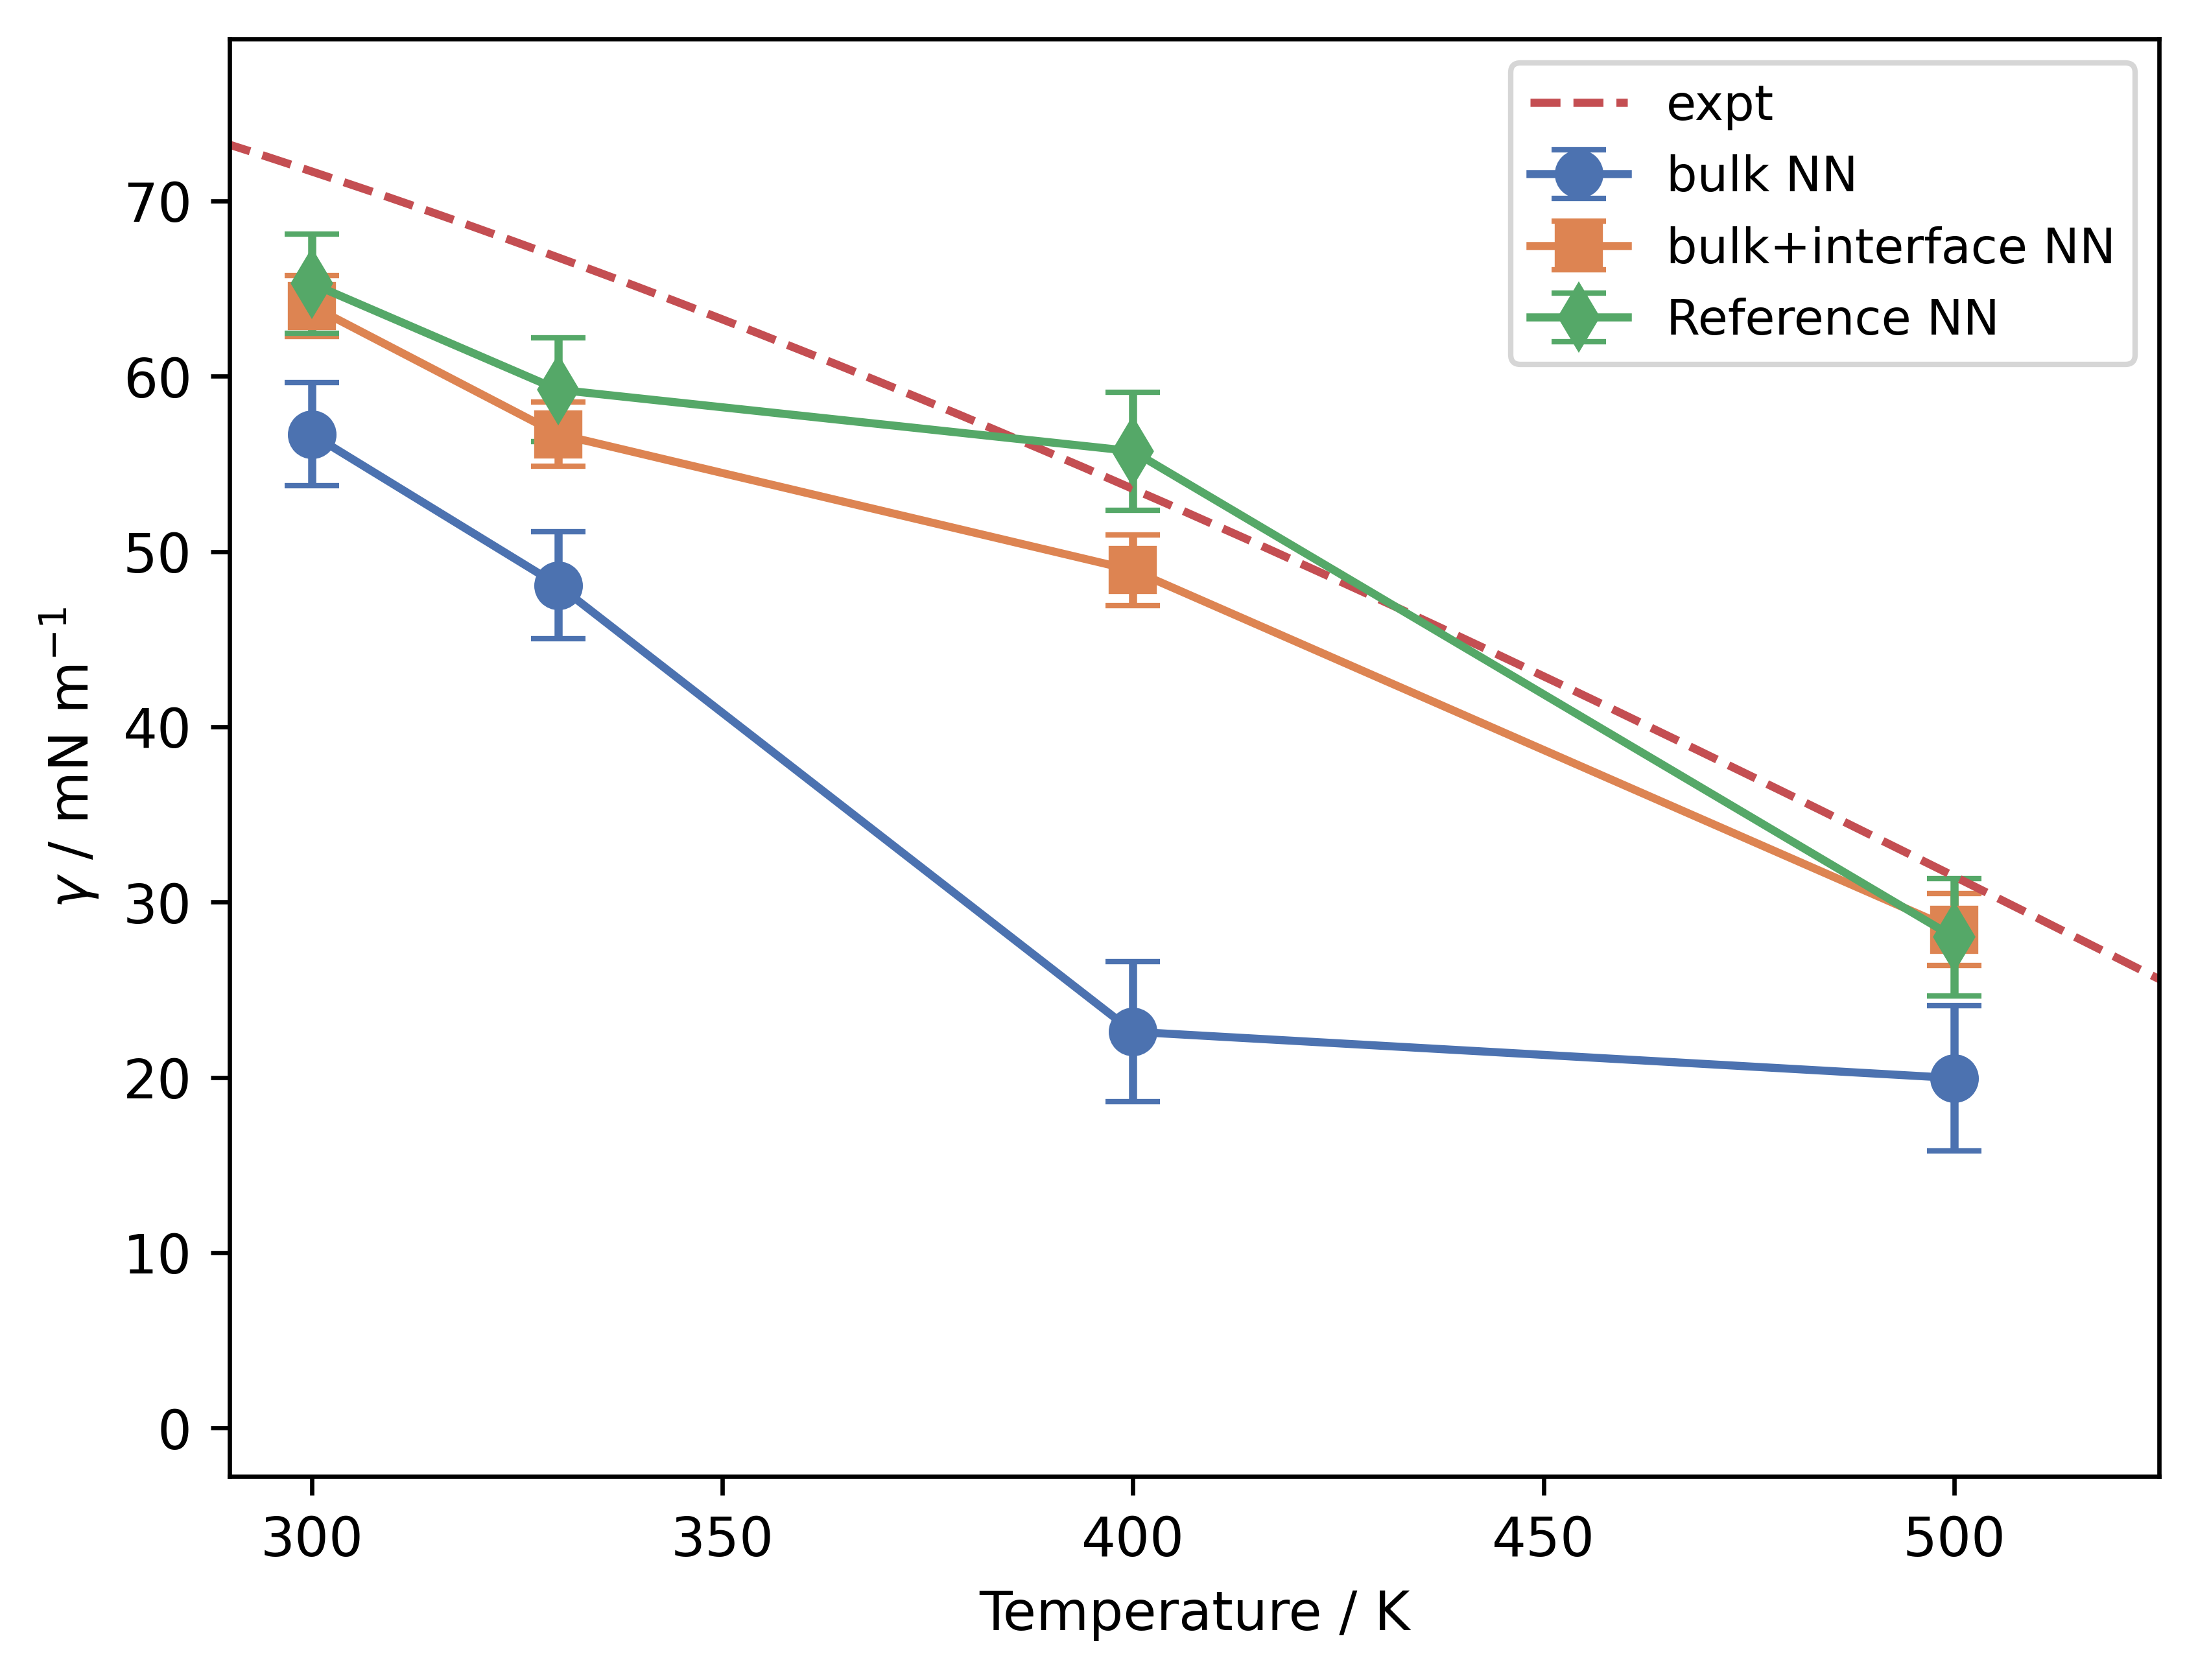
\includegraphics[width=0.7\linewidth]{images/surface_tension.png}
	\caption{Surface tension for different NNP models. The
		reference model is based on trained model of Sanchez-Burgos et
		al.~\cite{sanchez2023deep}.  }\label{fig:surf_tens}
\end{figure}

\section{Dipole Orientation}

One way to obtain microscopic properties of a system is by calculating the distribution of the average dipole moment orientation. Specifically, the $\cos(\theta)$ was computed, where $\theta$ is the angle between the dipole moment and the outward normal vector of the surface, as schematically shown in Figure~\ref{fig:dipole_scheme}. Positive values correspond to alignment of the dipole with the outward normal vector. Experimental techniques, such as vibrational sum frequency spectroscopy, have shown that the imaginary component of nonlinear susceptibility changes sign twice~\cite{fan2009structure}, implying a preferential orientation of water at the interface that forms two layers. As shown schematically in Figure\ref{fig:dipole_expt}, the water molecule in the first layer will align such that one of the OH bonds points toward the vapor phase. The net dipole moment from these covalent bonds will orient slightly towards the surface. Moreover, between the first and second layers, hydrogen bonds can produce an effective dipole moment in the opposite direction of the first layer. These are depicted as arrows in Figure~\ref{fig:dipole_guide}. Therefore, a flip in dipole orientation distribution at the interface is expected.

However, as shown in Figure~\ref{fig:dipole_orient}, only one type of orientation is observed for the different NNP models. The NNP model trained with both bulk and surface environments exhibits an opposite dipole orientation compared to models trained on bulk environments only. It can be hypothesized that the bulk+interface-trained NNP enhances dipoles pointing downward, while the bulk-trained NNP enhances dipoles pointing upward.

Additionally, it can be observed that the bulk region shows a nonzero dipole moment, which may be caused by the small system size, enhancing finite-size effects. Ideally, there should be zero net dipole moment inside the bulk due to the random thermal reorientation of water molecules and by symmetry.


\begin{figure}[tbhp!]
	\centering
	\begin{subfigure}{0.47\textwidth}
		\centering

		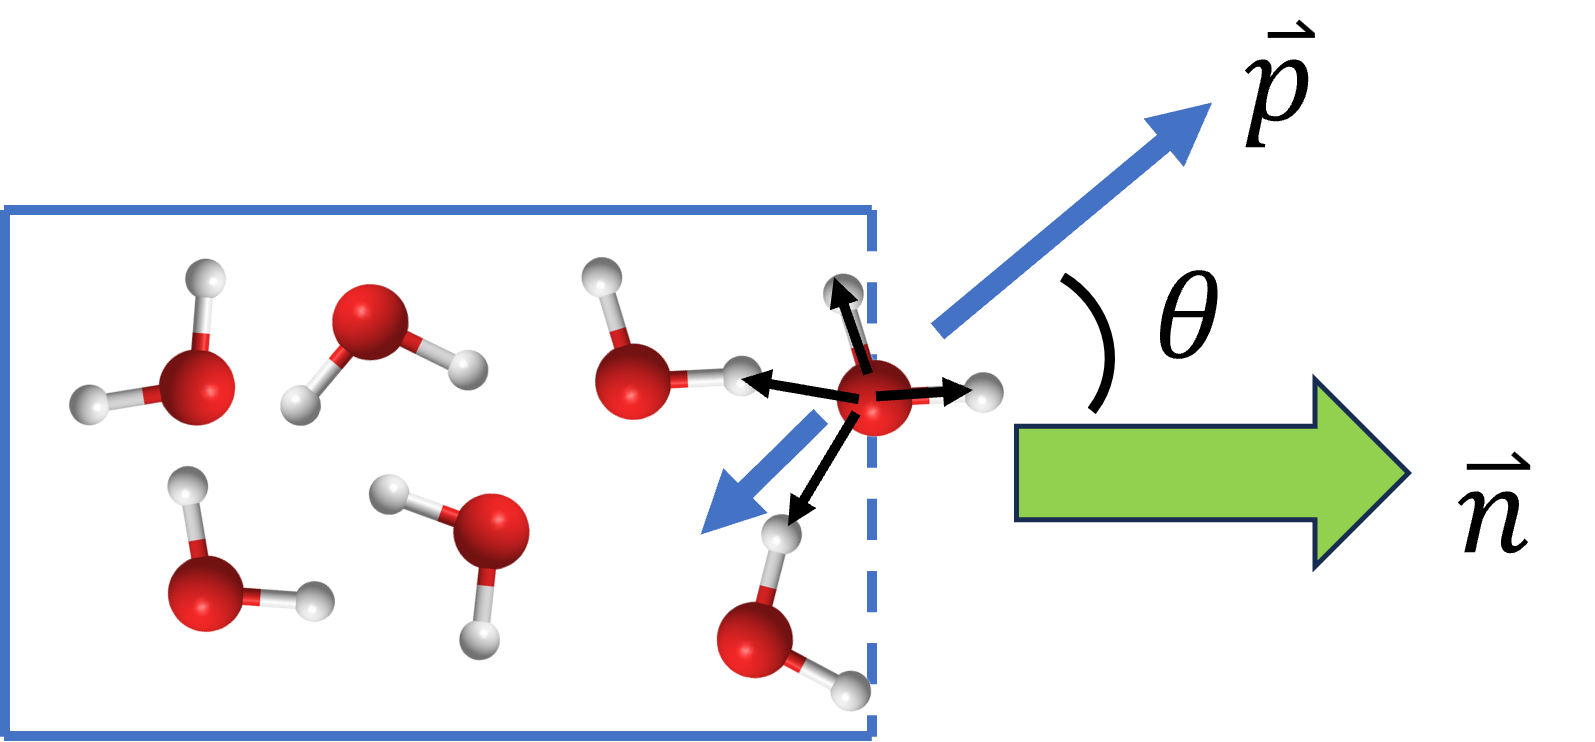
\includegraphics[width=0.9\textwidth]{images/dipole_scheme.png}
		\caption{}\label{fig:dipole_scheme}
	\end{subfigure}
	\hfill
	\begin{subfigure}{0.47\textwidth}
		\centering

		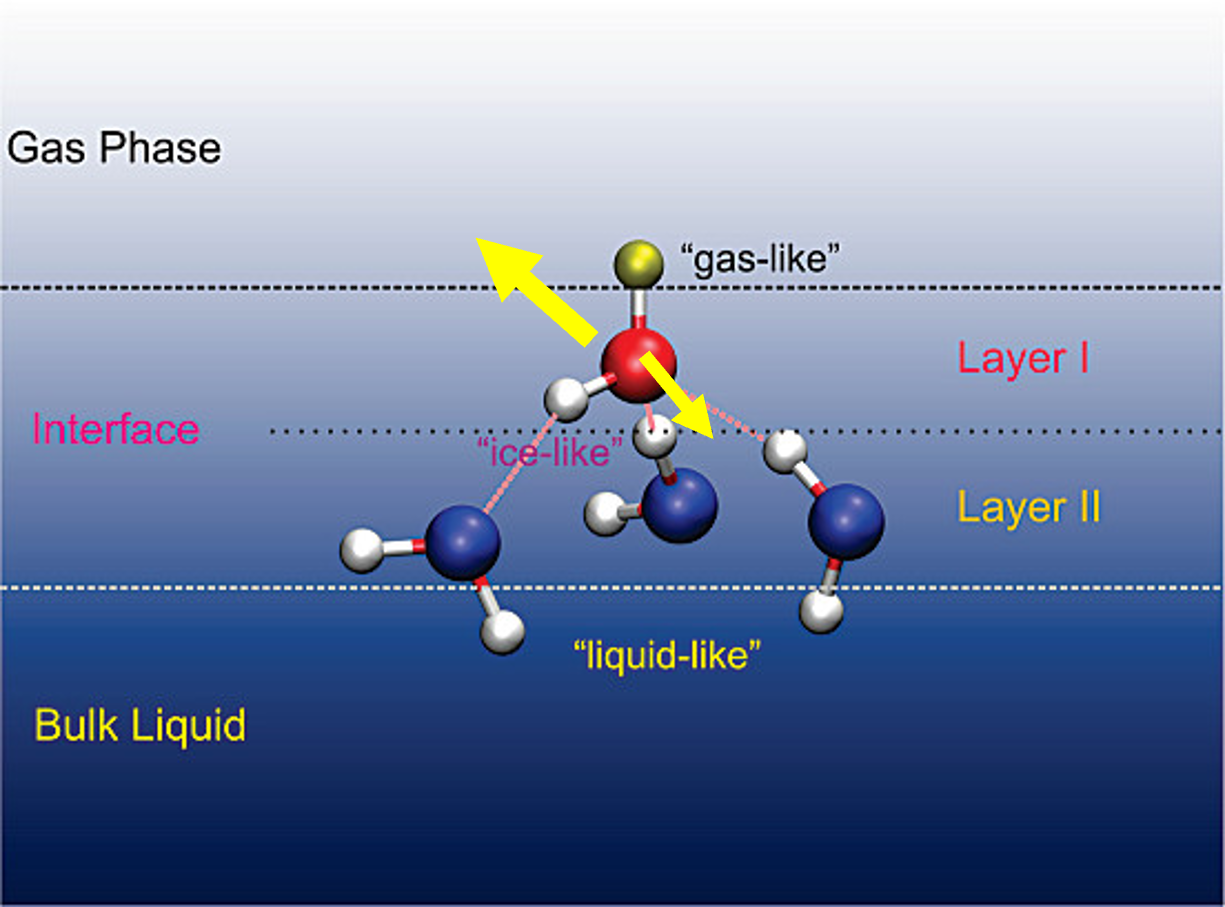
\includegraphics[width=0.9\textwidth]{images/dipole_expt.png}
		\caption{}\label{fig:dipole_expt}
	\end{subfigure}
	\caption{  Schematic diagram of the (a) dipole moment orientation and
		(b)		existence of two layers in the interface~\cite{fan2009structure}.}\label{fig:dipole_guide}
\end{figure}

\begin{figure}[tbhp!]
	\centering
	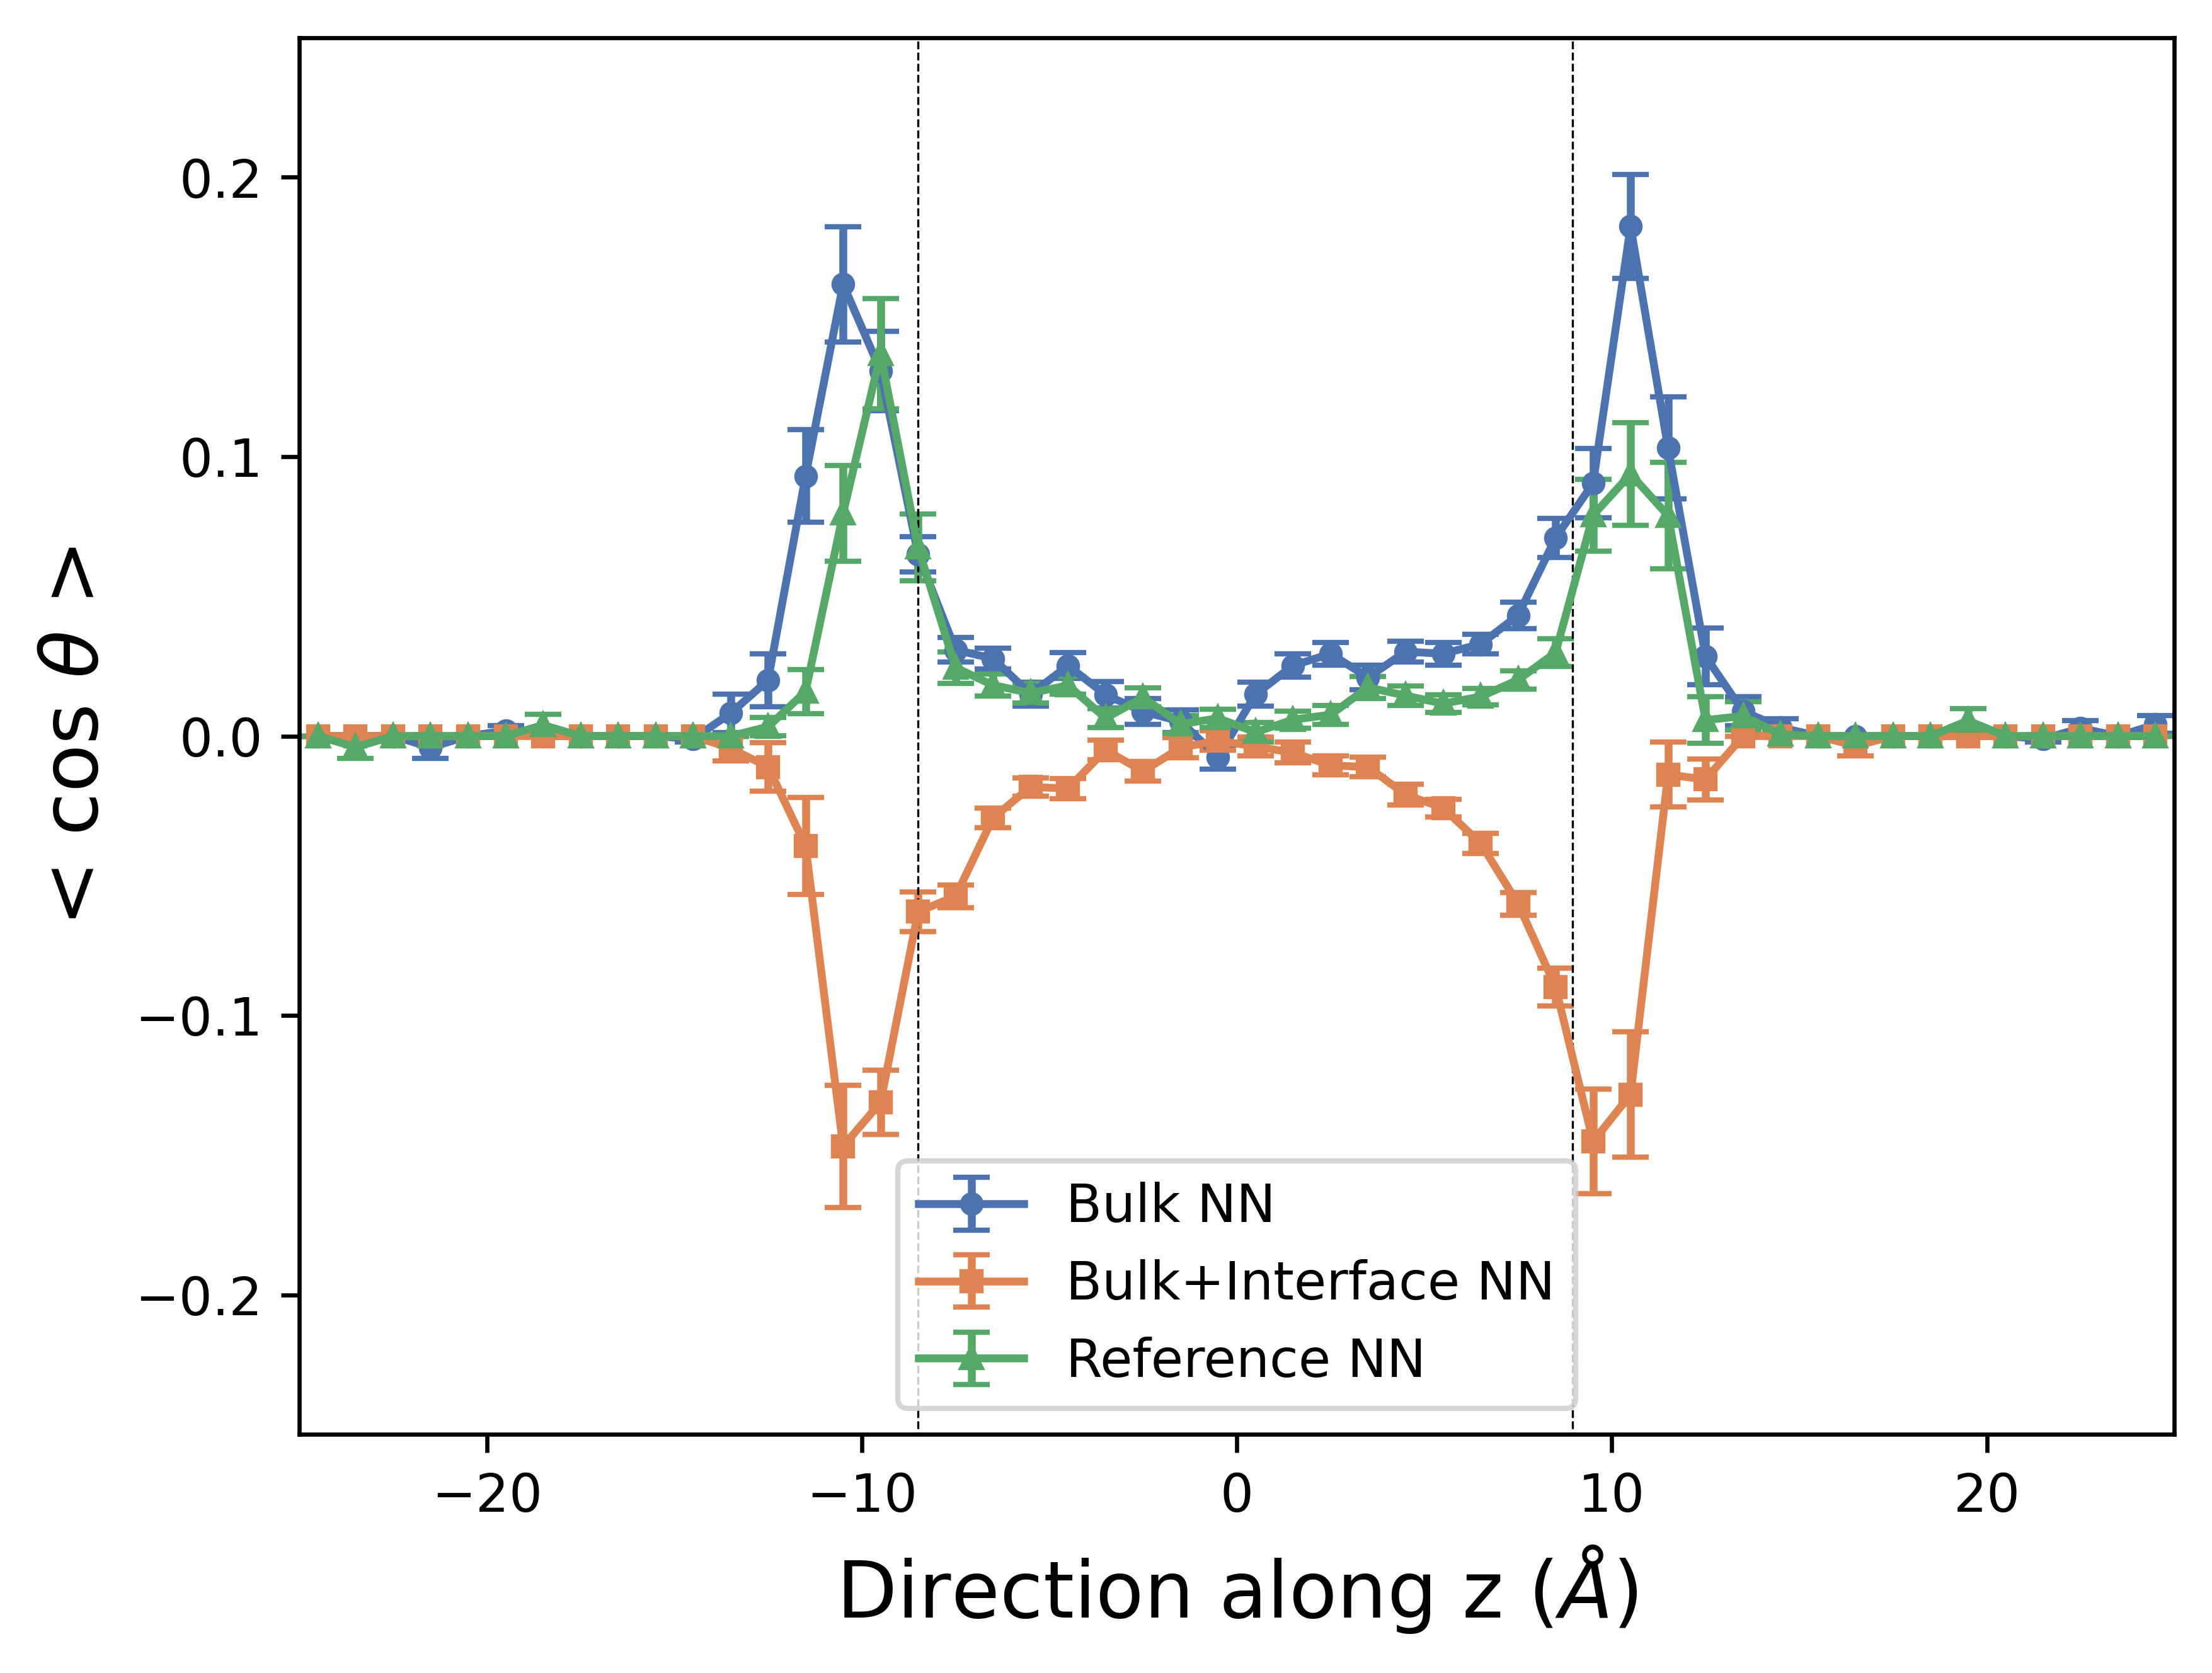
\includegraphics[width=0.75\linewidth]{images/dipole_dist_new.png}
	\caption{Dipole Orientation for different NN models. The outward normal
		vector was set along +z axis for both the top and bottom
		surface. The vertical
		lines
		are
		the Gibbs Dividing Surface in which the density is half of the
		bulk value.
	}\label{fig:dipole_orient}
\end{figure}


\clearpage
